\documentclass[12pt]{Latex/Classes/PhDthesisPSnPDF} 

% This file contains macros that can be called up from connected TeX files
% It helps to summarise repeated code, e.g. figure insertion (see below).

% insert a centered figure with caption and description
% parameters 1:filename, 2:title, 3:description and label
\newcommand{\figuremacro}[3]{
	\begin{figure}[htbp]
		\centering
		\includegraphics[width=1\textwidth]{#1}
		\caption[#2]{\textbf{#2} - #3}
		\label{#1}
	\end{figure}
}

% insert a centered figure with caption and description AND WIDTH
% parameters 1:filename, 2:title, 3:description and label, 4: textwidth
% textwidth 1 means as text, 0.5 means half the width of the text
\newcommand{\figuremacroW}[4]{
	\begin{figure}[htbp]
		\centering
		\includegraphics[width=#4\textwidth]{#1}
		\caption[#2]{\textbf{#2} - #3}
		\label{#1}
	\end{figure}
}

% inserts a figure with wrapped around text; only suitable for NARROW figs
% o is for outside on a double paged document; others: l, r, i(inside)
% text and figure will each be half of the document width
% note: long captions often crash with adjacent content; take care
% in general: above 2 macro produce more reliable layout
\newcommand{\figuremacroN}[3]{
	\begin{wrapfigure}{o}{0.5\textwidth}
		\centering
		\includegraphics[width=0.48\textwidth]{#1}
		\caption[#2]{{\small\textbf{#2} - #3}}
		\label{#1}
	\end{wrapfigure}
}

% predefined commands by Harish
\newcommand{\PdfPsText}[2]{
  \ifpdf
     #1
  \else
     #2
  \fi
}

\newcommand{\IncludeGraphicsH}[3]{
  \PdfPsText{\includegraphics[height=#2]{#1}}{\includegraphics[bb = #3, height=#2]{#1}}
}

\newcommand{\IncludeGraphicsW}[3]{
  \PdfPsText{\includegraphics[width=#2]{#1}}{\includegraphics[bb = #3, width=#2]{#1}}
}

\newcommand{\InsertFig}[3]{
  \begin{figure}[!htbp]
    \begin{center}
      \leavevmode
      #1
      \caption{#2}
      \label{#3}
    \end{center}
  \end{figure}
}


%%% Local Variables: 
%%% mode: latex
%%% TeX-master: "~/Documents/LaTeX/CUEDThesisPSnPDF/thesis"
%%% End: 


\usepackage{geometry} % Required to change the page size to A4
\geometry{a4paper} % Set the page size to be A4 as opposed to the default US Letter

\usepackage{graphicx} % Required for including pictures
\usepackage{float}
\usepackage{wrapfig} % Allows in-line images such as the example fish picture
\usepackage{caption}
\usepackage{amsmath}
\usepackage{slashbox}
\usepackage{caption}


\usepackage{lipsum} % Used for inserting dummy 'Lorem ipsum' text into the template

\linespread{1.2} % Line spacing

%\setlength\parindent{0pt} % Uncomment to remove all indentation from paragraphs

\graphicspath{{./Pictures/}} % Specifies the directory where pictures are stored

\usepackage{listings}
\usepackage{color}

\definecolor{dkgreen}{rgb}{0,0.6,0}
\definecolor{gray}{rgb}{0.5,0.5,0.5}
\definecolor{mauve}{rgb}{0.58,0,0.82}

\lstset{frame=tb,
  language=Java,
  aboveskip=3mm,
  belowskip=3mm,
  showstringspaces=false,
  columns=flexible,
  basicstyle={\small\ttfamily},
  numbers=none,
  numberstyle=\tiny\color{gray},
  keywordstyle=\color{blue},
  commentstyle=\color{dkgreen},
  stringstyle=\color{mauve},
  breaklines=true,
  breakatwhitespace=true
  tabsize=3
}

\begin{document}

\begin{titlepage}

\newcommand{\HRule}{\rule{\linewidth}{0.5mm}} % Defines a new command for the horizontal lines, change thickness here

\center % Center everything on the page

\textsc{\LARGE Carnegie Mellon University}\\[1.5cm] % Name of your university/college
\textsc{\Large Master of Science in Music and Technology}\\[0.5cm] % Major heading such as course name

\HRule \\[0.4cm]
{\large \bfseries A Music Player for the \\ Human Computer Music Performance Project}\\[0.4cm] % Title of your document
\HRule \\[1.5cm]

\begin{minipage}{0.4\textwidth}
\begin{flushleft} \large
\emph{Author:}\\
Dalong \textsc{Cheng} % Your name
\end{flushleft}
\end{minipage}
~
\begin{minipage}{0.4\textwidth}
\begin{flushright} \large
\emph{Supervisor:} \\
Roger \textsc{Dannenberg} \\ % Supervisor's Name
Richard \textsc{Stern} \\
Richard \textsc{Randall}
\end{flushright}
\end{minipage}\\[4cm]

{\large \today}\\[3cm] % Date, change the \today to a set date if you want to be precise

%\includegraphics{Logo}\\[1cm] % Include a department/university logo - this will require the graphicx package

\vfill % Fill the rest of the page with whitespace

%----------------------------------------------------------------------------------------
%	TABLE OF CONTENTS
%----------------------------------------------------------------------------------------
\end{titlepage}

\setcounter{page}{2}
\pagenumbering{roman}

\frontmatter
% Thesis Abstract -----------------------------------------------------
\begin{abstracts}
From computer instruments to computer accompaniment, from composition
systems to conducting systems, musicians have been interacting with
computers for many years. The Human Computer Music Performance (HCMP)
project aims to create a more autonomous ``artificial  performer'' that does
not require human input or adjustment. The heart of the HCMP project is the
development of an HCMP Player which is able to flexibly change the tempo and
communicate with other HCMP components.

The HCMP Player is designed and implemented with two goals in mind. The
first goal is to design a MIDI player which has an efficient time and space
tempo changing algorithm. The algorithm must process frequent tempo changes
during a performance and within bounded time periods. The second goal is to
clearly define a set of programming interfaces in the HCMP player, which can
be easily extended and used to coordinate the components of the HCMP
project. In this paper, I describe the development process of the HCMP
player, from design logic and code structure to general software
architecture, from implementation to a complete software testing plan.
Challenges, problems during development and key design logic behind the
implementation are also covered.
\end{abstracts}

% Thesis Acknowledgements ------------------------------------------------

%\begin{acknowledgementslong} %uncommenting this line, gives a different acknowledgements heading
\begin{acknowledgements}      %this creates the heading for the acknowlegments
I would like to express my appreciation to my advisory committee: 
Prof. Roger B. Dannenberg, Prof. Richard Stern and Prof. Richard Randall. 
Thanks for giving me the opportunity to be part of CMU Music Technology program. 
Special thanks to Professor Dannenberg for his time, patience, and understanding.
Professor Dannenberg, it always has been my honor and pleasure to work with you. 
\end{acknowledgements}
%\end{acknowledgmentslong}


\setcounter{secnumdepth}{3} % organisational level that receives a numbers
\setcounter{tocdepth}{3}    % print table of contents for level 3
\tableofcontents % Include a table of contents

\listoffigures	% print list of figures

\listoftables

\newpage % Begins the essay on a new page instead of on the same page as the table of contents 

%----------------------------------------------------------------------------------------
%	INTRODUCTION
%----------------------------------------------------------------------------------------

\pagestyle{headings}
\setcounter{page}{1}
\pagenumbering{arabic}

\mainmatter
\renewcommand{\chaptername}{} % uncomment to print only "1" not "Chapter 1"

%Example citation 
\chapter{Introduction}

% the code below specifies where the figures are stored
\ifpdf
    \graphicspath{{1_introduction/figures/PNG/}{1_introduction/figures/PDF/}{1_introduction/figures/}}
\else
    \graphicspath{{1_introduction/figures/EPS/}{1_introduction/figures/}}
\fi

\section{Overview}
Computers have been widely used in music performances for many years. Some
advanced systems use the computer as a independent module to replace a
single instrument in an orchestra. In popular music computers have proved
to be particularly successful. Both classical and popular music have many
opportunities for innovative applications used by highly intelligent and
coordinated computer music systems. With more powerful algorithms and more
advanced sensing devices, computer music systems have the potential to
replace musicians. In the future, computer music systems will inspire new 
musical directions based on new
capabilities and generate new concepts from new technologies.

Live popular music offers a wealth of opportunities for computing and music
research.  We term the integration of computers as independent autonomous
performers into popular live music performances as Human Computer Music
Performance (HCMP). In HCMP computers become more than instruments and are,
in some degree, seen as performers. To bring HCMP into the realm of popular
music performance, certain problems need to be solved. 

One problem is that
popular music is organized around a tight synchronization to beats and a
computer cannot reliably and efficiently adapt to human tempo variations.
Another significant problem is that an HCMP project is a large complex
system which contain many components, each one relying on the cooperation of several
different subcomponents to complete its task.

The motivation behind the HCMP Player is to provide a good solution to these
problems. When successful, the HCMP Player will display different
representations of music, work as an accompaniment  and quickly adjust its
tempo to follow the performer. A clearly defined programming interface is
also required in order to foster communication and cooperation with all
components within the system. To create such a player, we must coordinate
time between different media. We need at least two functional components,
one component working as ``backend'' and responsible for coordinating and
scheduling different music events, the other, working as ``frontend'', will
receive commands from the user or other components and dynamically adjust
play sequence and tempo based on those requests.

This paper begins with the role of the HCMP Player in the HCMP project. Then
the ``big picture of'' of the HCMP project will be discussed, followed by a
presentation of the individual HCMP components. Finally the question that how
does the HMCP Player fit into the whole picture will be addressed. In the
following three chapters design issues with the HCMP Player are addressed.
Each chapter approaches the problem from a different perspective. Chapter 2
describes the design of Graphic User Interface (GUI) of HCMP Player together
with a detailed explanation of all the GUI components' usage and function.
Chapter 3 describes the ``backend'' of the HCMP Player - the player engine,
and illustrates how the player engine cooperates and communicates with the
GUI to complete external requests. Chapter 4 addresses the network
communication problem between multiple players. A set of unified API is
defined to make the HCMP Player compatible with other components in the HCMP
project.  Chapter 5 describes the implementation details of the HCMP Player
and includes pseucode to provide a clear explanation of this. Chapter 6
focuses on the evaluation of the HCMP Player, a full list of feature points
will be given and a clear success criteria used to evaluate the HCMP Player
will be defined.  In chapter 7, I summarize my work and propose possible
future works.

\section{Background}

Before making a formal introduction to the background of HCMP Player. 
I would like to make short review of  
some existed human computer music systems. The most common use of computer in
music performance is through computer instruments, typically keyboards.
These, and other electronic instruments, are essentially substitutes for traditional
instruments and rely upon human musicians for their control and coordination with
other musicians. Many composers of interactive contemporary art music use computers
to generate music in real time, often in response to live performers.

Another meaningful use of computer in music is computer accompaniment system 
\cite{Roger:89}, 
whcih solves the synchronization problem by assuming a pre-determined 
score (music notation). During the performance, a performer expressively 
played music score, while the accompaniment system ``listen'' and analysis, 
then follows the performer 
in the score and synchronizes an accompaniment.

In live popular music peformance, computer is quite useful too.
The computer has had a significant
impact on popular music through drum machines, sequencers and loop-based
interfaces, but one can argue that popular music has adapted to new technology
rather than the other way around. The sound and beat of drum machines seems stiff,
mechanical, and monotonous to many musicians, but that became the trance-like
foundation of club dance music and other forms . Similarly, 
the inability of
sequencers and other beat-based software to “listen” to human musicians has led to
performances with click tracks in fixed media or simply a fixed drum track that live
musicians must follow. Ableton Live \cite{Ableton:2011} is an example of software that
uses a beat, measure, and section framework to synchronize music in live
performance, but the program is not well suited to adapting to the tempo of live
musicians. Robertson and Plumbley \cite{Robertson:2007} used a real-time beat 
tracker in
conjunction with Ableton Live software to synchronize pre-recorded music 
to a live drummer. This extension could be considered HCMP.
The table 1.1 summarize some of existed computer music systems and their usage.

\begin{table}[htdp]
\centering
\begin{tabular}{| p{5cm} | p{8cm} |} % ccc means 3 columns, all centered; alternatives are l, r

\hline
Computer Instruments & Direct physical interaction with virtual instruments \\

\hline 
Interactive Contemporary Art Music & Composed interactions; often unconstrained by
traditional harmony or rhythm.\\

\hline
Computer Accompaniment & score following synchronizes computer to live performer.\\

\hline
Fixed Media  & Many musical styles and formats. Live performers
synchronize to fixed recording.\\

\hline
Conducting System & Synchronize live computer performance by tapping or
gesturing beats. Best with “expressive”
traditional/classical music.\\
\hline
\end{tabular}
\caption[Computer Music Systems Summary]{Computer Music Systems Summary}
\label{latexin_genes} % label for cross-links with \ref{latexin_genes}
\end{table}

\section{Objective}
The objective of HCMP \cite{Dawen:2011} is to create an autonomous 
``artificial performer'' with the ability of a human-level musical performance. 
Hopefully, HCMP does not require a human operator's interfere, the system itself 
is designed to be adaptive and responsive. With sophisticated listening and sensing
component, HCMP is able to adjust related system parameters in real-time during 
performance. From functional perspective, we can divide HCMP into two main
categories: music preparation and music performance. Music preparation
part aims to work and understand with multiple music representations. Music
performance part is to deal with various issues regarding to question 
how to play music.     

An important component of the music performance part is the HCMP Player, 
which is able to flexibly  
adjust and respond to changes of music signal. Figure 1 illustrates relationship 
between scheduler, conductor and HCMP Plyaer. During performance, the HCMP Player will 
be controlled by conductor and constantly receive control messages 
from its conductor. In this project, I will design, implement the HCMP midi player 
for the HCMP project that is able to fully cooperate with conductor and scheduler.
\begin{figure}[H] % Example image
\center{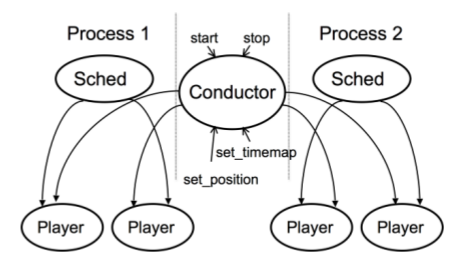
\includegraphics[width=0.65\linewidth]{1/1.png}}
\caption{Key Components of HCMP}
\label{fig:speciation}
\end{figure}
 

\section{Architecture}
\subsection{HCMP Architecture}
Figure 1.2 shows architecture of the whole HCMP project. it mainly contain 5 
subsystems. A brief description of each subsystem and its function will be
given in following paragraphs.
\begin{figure}[H] % Example image
\center{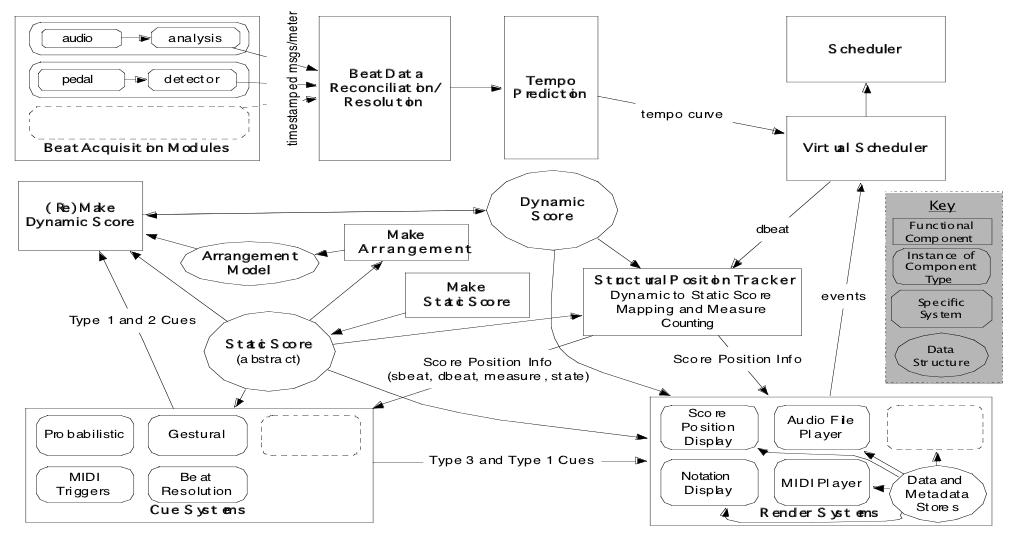
\includegraphics[width=1\linewidth]{1/2.png}}
\caption{Whole Picture of the HCMP Project}
\label{fig:speciation}
\end{figure}

\subsubsection{Real-Time System}
Real-time components are needed to keep an HCMP system coordinated with
the human musicians in an ensemble. Real-time synchronization aspects are
handled by components such as beat and tempo tracking systems.

\subsubsection{Abstract-Time System}
Abstract time components are needed to manage and schedule score events in
the context of the performance. The virtual scheduler and its associated systems are
concerned with the abstract time aspects of the system. The virtual scheduler should
reschedule events scheduled on a nominal time trajectory by warping the event times
according to the incoming tempo data from the tempo prediction system. Events are
then passed to an actual scheduler for real-time scheduling.

\subsubsection{Score and Arrangement System}
Score management is handled by the functional components in the center box of
the diagram. These systems will allow a human musician to encode, manage, and
arrange scores for performance.

\subsubsection{Cueing System}
Cueing systems are required to allow the computer system to react to high-level
structural and synchronization changes during performance (e.g. additional
repetitions of a chorus). There are mainly three types of cues:
\begin{enumerate}
  \item Static Score Position Cue. This cue is necessary when synchronization with the
static score is lost. Issuing it will cause the dynamic score to be re-made
accordingly.
  \item Intention Cue. This cue is needed to inform the computer of the intended
direction of the current performance (e.g. exiting a vamp section or adding an
additional chorus). Issuing it (e.g. using a MIDI trigger, gesture recognition or
other method) will cause the future dynamic score to be remade.
  \item Voicing/Arrangement Cue. This cue is needed to allow control over the voicing
of a section (e.g. it may be desirable to prevent a particular instrumental group
from playing on the first time through a repeat but allow them to play on the
second). Issuing this type of cue affects only the render system to which it is
issued.
\end{enumerate}

\subsubsection{Render System}
Render systems are responsible for providing different kindos multi-media output 
at the appropriate time. Render system will be designed as some kind of ``add-on'' 
for the HCMP, so that we could flexibly change, remove and update the render system.
With unified programming interface, each reander system is provided similar raw 
data and each system should also define its own way of parsing the raw data.
Sometimes, metadata is required to link these data elements to their appropriate 
static score position (and thus to
their appropriate scheduling as the dynamic score is played). A standardized
format will be required for this to relate static-score measure-numbers and the
dynamic score position and context to the properties of the format concerned. This
provide render systems more flexibility to determine how they need to deal with 
beat-level information or simply use the measure-level data, for example, a score 
display system might map a measure to image information or an audio render 
system might represent audio at the beat level.

%Abstract beat-time information can thus be linked to real-time source material
%(to allow the correct scheduling of real-time data) while allowing the overall system
%to remain oblivious to the specific source formats being used. Render systems
%should use a callback interface whereby they schedule events with the scheduling
%systems. These call the appropriate renderer at the scheduled time, causing
%synchronized real-time output of media in accordance with the dynamic score and
%beat tracking information.

\subsection{HCMP Player Architecture}
From system architectures' perspective, the interal HCMP Player is mainly made up of
two threads, we name the thread that taking
care of user input, maintaining graphic state GUI thread. And the thread worked as   
player engine is called performer thread, each thread is a independent 
module and executed in a separated thread space. Timer will be external source 
which periodically invoke the user in do some task. A timer usually come with a 
language library, so its implementation is within the category of this paper.

During the performance, the HCMP Player will act as 
the server for the conductor component, which is constantly 
receiving control messages and responding accordingly. 

\begin{figure}[H]
\center{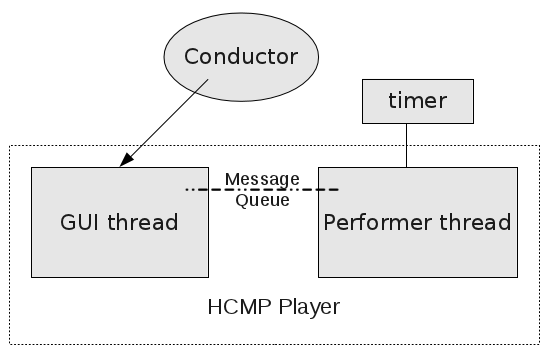
\includegraphics[width=0.65\linewidth]{2/2.png}}
\caption{Architecture of the HCMP Midi Player}
\label{fig:speciation}
\end{figure}

Internally, the Player will have two threads, with one thread for
GUI interactive control (GUI thread) and the other thread for 
performing music data (performer thread). 
The two threads will communicate with each other through a shared 
message queue, we can assume the message 
queue is large enough to avoid blocks for both caller and callee threads. 
The performaner thread
will handle time critical operations, and there will be a timer setup 
before this thread is created. The goal of the timer is to 
wake up the performer thread periodically. Everytime the performer 
thread's timer callback function is invoked, 
it will check the message queue and process any command from the control thread.
Figure 2 illustrates the overall structure of the Player.

%Most organisms use polymers of glucose units for energy storage and differ only slightly in the way they link together monomers to sometimes gigantic macromolecules. Dextran of bacteria is made from long chains of $\alpha$-1,6-linked glucose units. 

%: ----------------------- HELP: special characters
% above you can see how special characters are coded; e.g. $\alpha$
% below are the most frequently used codes:
%$\alpha$  $\beta$  $\gamma$  $\delta$

%$^{chars to be superscripted}$  OR $^x$ (for a single character)
%$_{chars to be suberscripted}$  OR $_x$

%>  $>$  greater,  <  $<$  less
%≥  $\ge$  greater than or equal, ≤  $\ge$  lesser than or equal
%~  $\sim$  similar to

%$^{\circ}$C   ° as in degree C
%±  \pm     plus/minus sign

%$\AA$     produces  Å (Angstrom)

% dextran, starch, glycogen continued
%Starch of plants and glycogen of animals consists of $\alpha$-1,4-glycosidic glucose polymers \cite{lastname07}. See figure \ref{largepotato} for a comparison of glucose polymer structure and chemistry. 

%Two references can be placed separated by a comma \cite{lastname07,name06}.

%: ----------------------- HELP: references
% References can be links to figures, tables, sections, or references.
% For figures, tables, and text you define the target of the link with \label{XYZ}. Then you call cross-link with the command \ref{XYZ}, as above
% Citations are bound in a very similar way with \cite{XYZ}. You store your references in a BibTex file with a programme like BibDesk.



%\figuremacro{largepotato}{A common glucose polymers}{The figure shows starch granules in potato cells, taken from \href{http://molecularexpressions.com/micro/gallery/burgersnfries/burgersnfries4.html}{Molecular Expressions}.}

%: ----------------------- HELP: adding figures with macros
% This template provides a very convenient way to add figures with minimal code.
% \figuremacro{1}{2}{3}{4} calls up a series of commands formating your image.
% 1 = name of the file without extension; PNG, JPEG is ok; GIF doesn't work
% 2 = title of the figure AND the name of the label for cross-linking
% 3 = caption text for the figure

%: ----------------------- HELP: www links
% You can also see above how, www links are placed
% \href{http://www.something.net}{link text}

%\figuremacroW{largepotato}{Title}{Caption}{0.8}

% variation of the above macro with a width setting
% \figuremacroW{1}{2}{3}{4}
% 1-3 as above
% 4 = size relative to text width which is 1; use this to reduce figures


%Insulin stimulates the following processes:
%
%\begin{itemize}
%\item muscle and fat cells remove glucose from the blood,
%\item cells breakdown glucose via glycolysis and the citrate cycle, storing its energy in the form of ATP,
%\item liver and muscle store glucose as glycogen as a short-term energy reserve,
%\item adipose tissue stores glucose as fat for long-term energy reserve, and
%\item cells use glucose for protein synthesis.
%\end{itemize}

%: ----------------------- HELP: lists
% This is how you generate lists in LaTeX.
% If you replace {itemize} by {enumerate} you get a numbered list.

%: ----------------------- HELP: tables
% Directly coding tables in latex is tiresome. See below.
% I would recommend using a converter macro that allows you to make the table in Excel and convert them into latex code which you can then paste into your doc.
% This is the link: http://www.softpedia.com/get/Office-tools/Other-Office-Tools/Excel2Latex.shtml
% It's a Excel template file containing a macro for the conversion.

% There you go. You already know the most important things.

\chapter{Introduction}

% the code below specifies where the figures are stored
\ifpdf
    \graphicspath{{1_introduction/figures/PNG/}{1_introduction/figures/PDF/}{1_introduction/figures/}}
\else
    \graphicspath{{1_introduction/figures/EPS/}{1_introduction/figures/}}
\fi

\section{Overview}
Computers have been widely used in music performances for many years. Some
advanced systems use the computer as a independent module to replace a
single instrument in an orchestra. In popular music computers have proved
to be particularly successful. Both classical and popular music have many
opportunities for innovative applications used by highly intelligent and
coordinated computer music systems. With more powerful algorithms and more
advanced sensing devices, computer music systems have the potential to
replace musicians. In the future, computer music systems will inspire new 
musical directions based on new
capabilities and generate new concepts from new technologies.

Live popular music offers a wealth of opportunities for computing and music
research.  We term the integration of computers as independent autonomous
performers into popular live music performances as Human Computer Music
Performance (HCMP). In HCMP computers become more than instruments and are,
in some degree, seen as performers. To bring HCMP into the realm of popular
music performance, certain problems need to be solved. 

One problem is that
popular music is organized around a tight synchronization to beats and a
computer cannot reliably and efficiently adapt to human tempo variations.
Another significant problem is that an HCMP project is a large complex
system which contain many components, each one relying on the cooperation of several
different subcomponents to complete its task.

The motivation behind the HCMP Player is to provide a good solution to these
problems. When successful, the HCMP Player will display different
representations of music, work as an accompaniment  and quickly adjust its
tempo to follow the performer. A clearly defined programming interface is
also required in order to foster communication and cooperation with all
components within the system. To create such a player, we must coordinate
time between different media. We need at least two functional components,
one component working as ``backend'' and responsible for coordinating and
scheduling different music events, the other, working as ``frontend'', will
receive commands from the user or other components and dynamically adjust
play sequence and tempo based on those requests.

This paper begins with the role of the HCMP Player in the HCMP project. Then
the ``big picture of'' of the HCMP project will be discussed, followed by a
presentation of the individual HCMP components. Finally the question that how
does the HMCP Player fit into the whole picture will be addressed. In the
following three chapters design issues with the HCMP Player are addressed.
Each chapter approaches the problem from a different perspective. Chapter 2
describes the design of Graphic User Interface (GUI) of HCMP Player together
with a detailed explanation of all the GUI components' usage and function.
Chapter 3 describes the ``backend'' of the HCMP Player - the player engine,
and illustrates how the player engine cooperates and communicates with the
GUI to complete external requests. Chapter 4 addresses the network
communication problem between multiple players. A set of unified API is
defined to make the HCMP Player compatible with other components in the HCMP
project.  Chapter 5 describes the implementation details of the HCMP Player
and includes pseucode to provide a clear explanation of this. Chapter 6
focuses on the evaluation of the HCMP Player, a full list of feature points
will be given and a clear success criteria used to evaluate the HCMP Player
will be defined.  In chapter 7, I summarize my work and propose possible
future works.

\section{Background}

Before making a formal introduction to the background of HCMP Player. 
I would like to make short review of  
some existed human computer music systems. The most common use of computer in
music performance is through computer instruments, typically keyboards.
These, and other electronic instruments, are essentially substitutes for traditional
instruments and rely upon human musicians for their control and coordination with
other musicians. Many composers of interactive contemporary art music use computers
to generate music in real time, often in response to live performers.

Another meaningful use of computer in music is computer accompaniment system 
\cite{Roger:89}, 
whcih solves the synchronization problem by assuming a pre-determined 
score (music notation). During the performance, a performer expressively 
played music score, while the accompaniment system ``listen'' and analysis, 
then follows the performer 
in the score and synchronizes an accompaniment.

In live popular music peformance, computer is quite useful too.
The computer has had a significant
impact on popular music through drum machines, sequencers and loop-based
interfaces, but one can argue that popular music has adapted to new technology
rather than the other way around. The sound and beat of drum machines seems stiff,
mechanical, and monotonous to many musicians, but that became the trance-like
foundation of club dance music and other forms . Similarly, 
the inability of
sequencers and other beat-based software to “listen” to human musicians has led to
performances with click tracks in fixed media or simply a fixed drum track that live
musicians must follow. Ableton Live \cite{Ableton:2011} is an example of software that
uses a beat, measure, and section framework to synchronize music in live
performance, but the program is not well suited to adapting to the tempo of live
musicians. Robertson and Plumbley \cite{Robertson:2007} used a real-time beat 
tracker in
conjunction with Ableton Live software to synchronize pre-recorded music 
to a live drummer. This extension could be considered HCMP.
The table 1.1 summarize some of existed computer music systems and their usage.

\begin{table}[htdp]
\centering
\begin{tabular}{| p{5cm} | p{8cm} |} % ccc means 3 columns, all centered; alternatives are l, r

\hline
Computer Instruments & Direct physical interaction with virtual instruments \\

\hline 
Interactive Contemporary Art Music & Composed interactions; often unconstrained by
traditional harmony or rhythm.\\

\hline
Computer Accompaniment & score following synchronizes computer to live performer.\\

\hline
Fixed Media  & Many musical styles and formats. Live performers
synchronize to fixed recording.\\

\hline
Conducting System & Synchronize live computer performance by tapping or
gesturing beats. Best with “expressive”
traditional/classical music.\\
\hline
\end{tabular}
\caption[Computer Music Systems Summary]{Computer Music Systems Summary}
\label{latexin_genes} % label for cross-links with \ref{latexin_genes}
\end{table}

\section{Objective}
The objective of HCMP \cite{Dawen:2011} is to create an autonomous 
``artificial performer'' with the ability of a human-level musical performance. 
Hopefully, HCMP does not require a human operator's interfere, the system itself 
is designed to be adaptive and responsive. With sophisticated listening and sensing
component, HCMP is able to adjust related system parameters in real-time during 
performance. From functional perspective, we can divide HCMP into two main
categories: music preparation and music performance. Music preparation
part aims to work and understand with multiple music representations. Music
performance part is to deal with various issues regarding to question 
how to play music.     

An important component of the music performance part is the HCMP Player, 
which is able to flexibly  
adjust and respond to changes of music signal. Figure 1 illustrates relationship 
between scheduler, conductor and HCMP Plyaer. During performance, the HCMP Player will 
be controlled by conductor and constantly receive control messages 
from its conductor. In this project, I will design, implement the HCMP midi player 
for the HCMP project that is able to fully cooperate with conductor and scheduler.
\begin{figure}[H] % Example image
\center{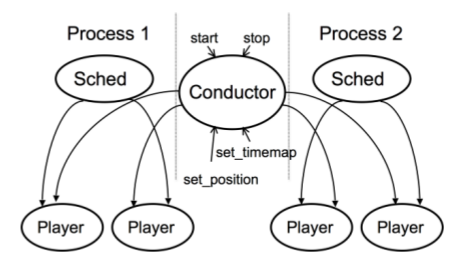
\includegraphics[width=0.65\linewidth]{1/1.png}}
\caption{Key Components of HCMP}
\label{fig:speciation}
\end{figure}
 

\section{Architecture}
\subsection{HCMP Architecture}
Figure 1.2 shows architecture of the whole HCMP project. it mainly contain 5 
subsystems. A brief description of each subsystem and its function will be
given in following paragraphs.
\begin{figure}[H] % Example image
\center{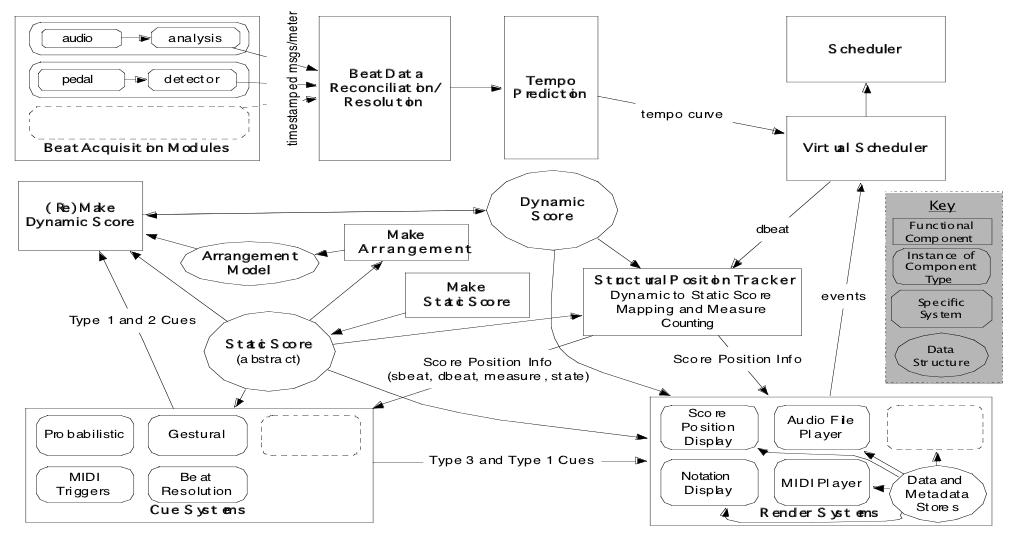
\includegraphics[width=1\linewidth]{1/2.png}}
\caption{Whole Picture of the HCMP Project}
\label{fig:speciation}
\end{figure}

\subsubsection{Real-Time System}
Real-time components are needed to keep an HCMP system coordinated with
the human musicians in an ensemble. Real-time synchronization aspects are
handled by components such as beat and tempo tracking systems.

\subsubsection{Abstract-Time System}
Abstract time components are needed to manage and schedule score events in
the context of the performance. The virtual scheduler and its associated systems are
concerned with the abstract time aspects of the system. The virtual scheduler should
reschedule events scheduled on a nominal time trajectory by warping the event times
according to the incoming tempo data from the tempo prediction system. Events are
then passed to an actual scheduler for real-time scheduling.

\subsubsection{Score and Arrangement System}
Score management is handled by the functional components in the center box of
the diagram. These systems will allow a human musician to encode, manage, and
arrange scores for performance.

\subsubsection{Cueing System}
Cueing systems are required to allow the computer system to react to high-level
structural and synchronization changes during performance (e.g. additional
repetitions of a chorus). There are mainly three types of cues:
\begin{enumerate}
  \item Static Score Position Cue. This cue is necessary when synchronization with the
static score is lost. Issuing it will cause the dynamic score to be re-made
accordingly.
  \item Intention Cue. This cue is needed to inform the computer of the intended
direction of the current performance (e.g. exiting a vamp section or adding an
additional chorus). Issuing it (e.g. using a MIDI trigger, gesture recognition or
other method) will cause the future dynamic score to be remade.
  \item Voicing/Arrangement Cue. This cue is needed to allow control over the voicing
of a section (e.g. it may be desirable to prevent a particular instrumental group
from playing on the first time through a repeat but allow them to play on the
second). Issuing this type of cue affects only the render system to which it is
issued.
\end{enumerate}

\subsubsection{Render System}
Render systems are responsible for providing different kindos multi-media output 
at the appropriate time. Render system will be designed as some kind of ``add-on'' 
for the HCMP, so that we could flexibly change, remove and update the render system.
With unified programming interface, each reander system is provided similar raw 
data and each system should also define its own way of parsing the raw data.
Sometimes, metadata is required to link these data elements to their appropriate 
static score position (and thus to
their appropriate scheduling as the dynamic score is played). A standardized
format will be required for this to relate static-score measure-numbers and the
dynamic score position and context to the properties of the format concerned. This
provide render systems more flexibility to determine how they need to deal with 
beat-level information or simply use the measure-level data, for example, a score 
display system might map a measure to image information or an audio render 
system might represent audio at the beat level.

%Abstract beat-time information can thus be linked to real-time source material
%(to allow the correct scheduling of real-time data) while allowing the overall system
%to remain oblivious to the specific source formats being used. Render systems
%should use a callback interface whereby they schedule events with the scheduling
%systems. These call the appropriate renderer at the scheduled time, causing
%synchronized real-time output of media in accordance with the dynamic score and
%beat tracking information.

\subsection{HCMP Player Architecture}
From system architectures' perspective, the interal HCMP Player is mainly made up of
two threads, we name the thread that taking
care of user input, maintaining graphic state GUI thread. And the thread worked as   
player engine is called performer thread, each thread is a independent 
module and executed in a separated thread space. Timer will be external source 
which periodically invoke the user in do some task. A timer usually come with a 
language library, so its implementation is within the category of this paper.

During the performance, the HCMP Player will act as 
the server for the conductor component, which is constantly 
receiving control messages and responding accordingly. 

\begin{figure}[H]
\center{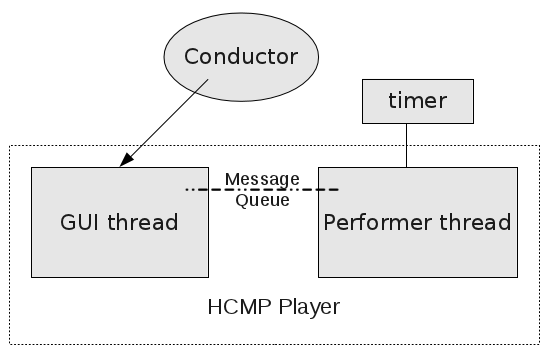
\includegraphics[width=0.65\linewidth]{2/2.png}}
\caption{Architecture of the HCMP Midi Player}
\label{fig:speciation}
\end{figure}

Internally, the Player will have two threads, with one thread for
GUI interactive control (GUI thread) and the other thread for 
performing music data (performer thread). 
The two threads will communicate with each other through a shared 
message queue, we can assume the message 
queue is large enough to avoid blocks for both caller and callee threads. 
The performaner thread
will handle time critical operations, and there will be a timer setup 
before this thread is created. The goal of the timer is to 
wake up the performer thread periodically. Everytime the performer 
thread's timer callback function is invoked, 
it will check the message queue and process any command from the control thread.
Figure 2 illustrates the overall structure of the Player.

%Most organisms use polymers of glucose units for energy storage and differ only slightly in the way they link together monomers to sometimes gigantic macromolecules. Dextran of bacteria is made from long chains of $\alpha$-1,6-linked glucose units. 

%: ----------------------- HELP: special characters
% above you can see how special characters are coded; e.g. $\alpha$
% below are the most frequently used codes:
%$\alpha$  $\beta$  $\gamma$  $\delta$

%$^{chars to be superscripted}$  OR $^x$ (for a single character)
%$_{chars to be suberscripted}$  OR $_x$

%>  $>$  greater,  <  $<$  less
%≥  $\ge$  greater than or equal, ≤  $\ge$  lesser than or equal
%~  $\sim$  similar to

%$^{\circ}$C   ° as in degree C
%±  \pm     plus/minus sign

%$\AA$     produces  Å (Angstrom)

% dextran, starch, glycogen continued
%Starch of plants and glycogen of animals consists of $\alpha$-1,4-glycosidic glucose polymers \cite{lastname07}. See figure \ref{largepotato} for a comparison of glucose polymer structure and chemistry. 

%Two references can be placed separated by a comma \cite{lastname07,name06}.

%: ----------------------- HELP: references
% References can be links to figures, tables, sections, or references.
% For figures, tables, and text you define the target of the link with \label{XYZ}. Then you call cross-link with the command \ref{XYZ}, as above
% Citations are bound in a very similar way with \cite{XYZ}. You store your references in a BibTex file with a programme like BibDesk.



%\figuremacro{largepotato}{A common glucose polymers}{The figure shows starch granules in potato cells, taken from \href{http://molecularexpressions.com/micro/gallery/burgersnfries/burgersnfries4.html}{Molecular Expressions}.}

%: ----------------------- HELP: adding figures with macros
% This template provides a very convenient way to add figures with minimal code.
% \figuremacro{1}{2}{3}{4} calls up a series of commands formating your image.
% 1 = name of the file without extension; PNG, JPEG is ok; GIF doesn't work
% 2 = title of the figure AND the name of the label for cross-linking
% 3 = caption text for the figure

%: ----------------------- HELP: www links
% You can also see above how, www links are placed
% \href{http://www.something.net}{link text}

%\figuremacroW{largepotato}{Title}{Caption}{0.8}

% variation of the above macro with a width setting
% \figuremacroW{1}{2}{3}{4}
% 1-3 as above
% 4 = size relative to text width which is 1; use this to reduce figures


%Insulin stimulates the following processes:
%
%\begin{itemize}
%\item muscle and fat cells remove glucose from the blood,
%\item cells breakdown glucose via glycolysis and the citrate cycle, storing its energy in the form of ATP,
%\item liver and muscle store glucose as glycogen as a short-term energy reserve,
%\item adipose tissue stores glucose as fat for long-term energy reserve, and
%\item cells use glucose for protein synthesis.
%\end{itemize}

%: ----------------------- HELP: lists
% This is how you generate lists in LaTeX.
% If you replace {itemize} by {enumerate} you get a numbered list.

%: ----------------------- HELP: tables
% Directly coding tables in latex is tiresome. See below.
% I would recommend using a converter macro that allows you to make the table in Excel and convert them into latex code which you can then paste into your doc.
% This is the link: http://www.softpedia.com/get/Office-tools/Other-Office-Tools/Excel2Latex.shtml
% It's a Excel template file containing a macro for the conversion.

% There you go. You already know the most important things.

\chapter{Introduction}

% the code below specifies where the figures are stored
\ifpdf
    \graphicspath{{1_introduction/figures/PNG/}{1_introduction/figures/PDF/}{1_introduction/figures/}}
\else
    \graphicspath{{1_introduction/figures/EPS/}{1_introduction/figures/}}
\fi

\section{Overview}
Computers have been widely used in music performances for many years. Some
advanced systems use the computer as a independent module to replace a
single instrument in an orchestra. In popular music computers have proved
to be particularly successful. Both classical and popular music have many
opportunities for innovative applications used by highly intelligent and
coordinated computer music systems. With more powerful algorithms and more
advanced sensing devices, computer music systems have the potential to
replace musicians. In the future, computer music systems will inspire new 
musical directions based on new
capabilities and generate new concepts from new technologies.

Live popular music offers a wealth of opportunities for computing and music
research.  We term the integration of computers as independent autonomous
performers into popular live music performances as Human Computer Music
Performance (HCMP). In HCMP computers become more than instruments and are,
in some degree, seen as performers. To bring HCMP into the realm of popular
music performance, certain problems need to be solved. 

One problem is that
popular music is organized around a tight synchronization to beats and a
computer cannot reliably and efficiently adapt to human tempo variations.
Another significant problem is that an HCMP project is a large complex
system which contain many components, each one relying on the cooperation of several
different subcomponents to complete its task.

The motivation behind the HCMP Player is to provide a good solution to these
problems. When successful, the HCMP Player will display different
representations of music, work as an accompaniment  and quickly adjust its
tempo to follow the performer. A clearly defined programming interface is
also required in order to foster communication and cooperation with all
components within the system. To create such a player, we must coordinate
time between different media. We need at least two functional components,
one component working as ``backend'' and responsible for coordinating and
scheduling different music events, the other, working as ``frontend'', will
receive commands from the user or other components and dynamically adjust
play sequence and tempo based on those requests.

This paper begins with the role of the HCMP Player in the HCMP project. Then
the ``big picture of'' of the HCMP project will be discussed, followed by a
presentation of the individual HCMP components. Finally the question that how
does the HMCP Player fit into the whole picture will be addressed. In the
following three chapters design issues with the HCMP Player are addressed.
Each chapter approaches the problem from a different perspective. Chapter 2
describes the design of Graphic User Interface (GUI) of HCMP Player together
with a detailed explanation of all the GUI components' usage and function.
Chapter 3 describes the ``backend'' of the HCMP Player - the player engine,
and illustrates how the player engine cooperates and communicates with the
GUI to complete external requests. Chapter 4 addresses the network
communication problem between multiple players. A set of unified API is
defined to make the HCMP Player compatible with other components in the HCMP
project.  Chapter 5 describes the implementation details of the HCMP Player
and includes pseucode to provide a clear explanation of this. Chapter 6
focuses on the evaluation of the HCMP Player, a full list of feature points
will be given and a clear success criteria used to evaluate the HCMP Player
will be defined.  In chapter 7, I summarize my work and propose possible
future works.

\section{Background}

Before making a formal introduction to the background of HCMP Player. 
I would like to make short review of  
some existed human computer music systems. The most common use of computer in
music performance is through computer instruments, typically keyboards.
These, and other electronic instruments, are essentially substitutes for traditional
instruments and rely upon human musicians for their control and coordination with
other musicians. Many composers of interactive contemporary art music use computers
to generate music in real time, often in response to live performers.

Another meaningful use of computer in music is computer accompaniment system 
\cite{Roger:89}, 
whcih solves the synchronization problem by assuming a pre-determined 
score (music notation). During the performance, a performer expressively 
played music score, while the accompaniment system ``listen'' and analysis, 
then follows the performer 
in the score and synchronizes an accompaniment.

In live popular music peformance, computer is quite useful too.
The computer has had a significant
impact on popular music through drum machines, sequencers and loop-based
interfaces, but one can argue that popular music has adapted to new technology
rather than the other way around. The sound and beat of drum machines seems stiff,
mechanical, and monotonous to many musicians, but that became the trance-like
foundation of club dance music and other forms . Similarly, 
the inability of
sequencers and other beat-based software to “listen” to human musicians has led to
performances with click tracks in fixed media or simply a fixed drum track that live
musicians must follow. Ableton Live \cite{Ableton:2011} is an example of software that
uses a beat, measure, and section framework to synchronize music in live
performance, but the program is not well suited to adapting to the tempo of live
musicians. Robertson and Plumbley \cite{Robertson:2007} used a real-time beat 
tracker in
conjunction with Ableton Live software to synchronize pre-recorded music 
to a live drummer. This extension could be considered HCMP.
The table 1.1 summarize some of existed computer music systems and their usage.

\begin{table}[htdp]
\centering
\begin{tabular}{| p{5cm} | p{8cm} |} % ccc means 3 columns, all centered; alternatives are l, r

\hline
Computer Instruments & Direct physical interaction with virtual instruments \\

\hline 
Interactive Contemporary Art Music & Composed interactions; often unconstrained by
traditional harmony or rhythm.\\

\hline
Computer Accompaniment & score following synchronizes computer to live performer.\\

\hline
Fixed Media  & Many musical styles and formats. Live performers
synchronize to fixed recording.\\

\hline
Conducting System & Synchronize live computer performance by tapping or
gesturing beats. Best with “expressive”
traditional/classical music.\\
\hline
\end{tabular}
\caption[Computer Music Systems Summary]{Computer Music Systems Summary}
\label{latexin_genes} % label for cross-links with \ref{latexin_genes}
\end{table}

\section{Objective}
The objective of HCMP \cite{Dawen:2011} is to create an autonomous 
``artificial performer'' with the ability of a human-level musical performance. 
Hopefully, HCMP does not require a human operator's interfere, the system itself 
is designed to be adaptive and responsive. With sophisticated listening and sensing
component, HCMP is able to adjust related system parameters in real-time during 
performance. From functional perspective, we can divide HCMP into two main
categories: music preparation and music performance. Music preparation
part aims to work and understand with multiple music representations. Music
performance part is to deal with various issues regarding to question 
how to play music.     

An important component of the music performance part is the HCMP Player, 
which is able to flexibly  
adjust and respond to changes of music signal. Figure 1 illustrates relationship 
between scheduler, conductor and HCMP Plyaer. During performance, the HCMP Player will 
be controlled by conductor and constantly receive control messages 
from its conductor. In this project, I will design, implement the HCMP midi player 
for the HCMP project that is able to fully cooperate with conductor and scheduler.
\begin{figure}[H] % Example image
\center{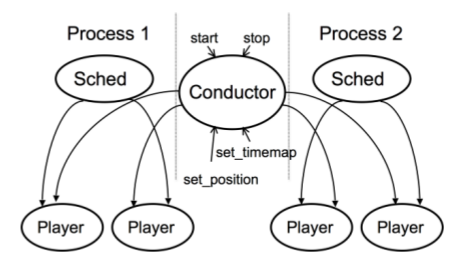
\includegraphics[width=0.65\linewidth]{1/1.png}}
\caption{Key Components of HCMP}
\label{fig:speciation}
\end{figure}
 

\section{Architecture}
\subsection{HCMP Architecture}
Figure 1.2 shows architecture of the whole HCMP project. it mainly contain 5 
subsystems. A brief description of each subsystem and its function will be
given in following paragraphs.
\begin{figure}[H] % Example image
\center{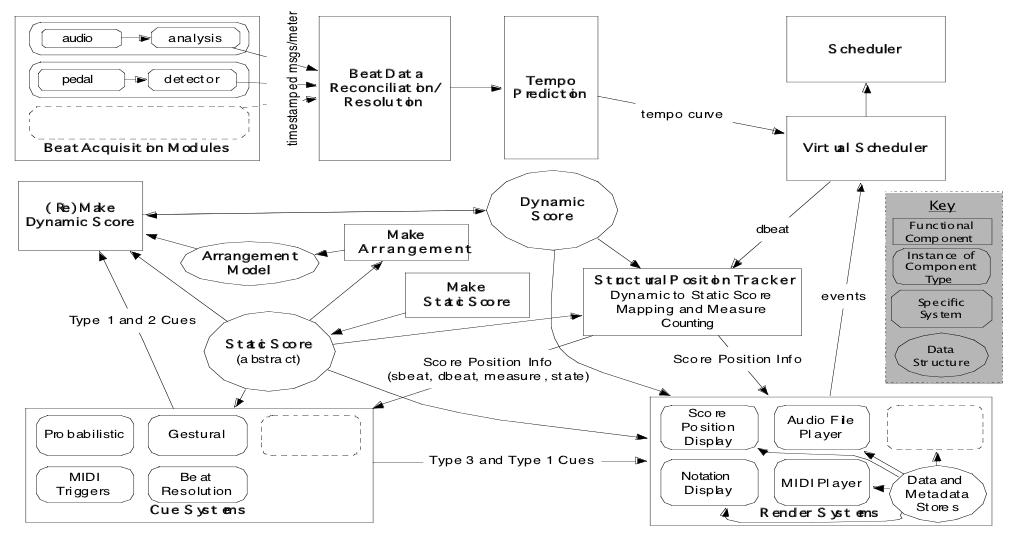
\includegraphics[width=1\linewidth]{1/2.png}}
\caption{Whole Picture of the HCMP Project}
\label{fig:speciation}
\end{figure}

\subsubsection{Real-Time System}
Real-time components are needed to keep an HCMP system coordinated with
the human musicians in an ensemble. Real-time synchronization aspects are
handled by components such as beat and tempo tracking systems.

\subsubsection{Abstract-Time System}
Abstract time components are needed to manage and schedule score events in
the context of the performance. The virtual scheduler and its associated systems are
concerned with the abstract time aspects of the system. The virtual scheduler should
reschedule events scheduled on a nominal time trajectory by warping the event times
according to the incoming tempo data from the tempo prediction system. Events are
then passed to an actual scheduler for real-time scheduling.

\subsubsection{Score and Arrangement System}
Score management is handled by the functional components in the center box of
the diagram. These systems will allow a human musician to encode, manage, and
arrange scores for performance.

\subsubsection{Cueing System}
Cueing systems are required to allow the computer system to react to high-level
structural and synchronization changes during performance (e.g. additional
repetitions of a chorus). There are mainly three types of cues:
\begin{enumerate}
  \item Static Score Position Cue. This cue is necessary when synchronization with the
static score is lost. Issuing it will cause the dynamic score to be re-made
accordingly.
  \item Intention Cue. This cue is needed to inform the computer of the intended
direction of the current performance (e.g. exiting a vamp section or adding an
additional chorus). Issuing it (e.g. using a MIDI trigger, gesture recognition or
other method) will cause the future dynamic score to be remade.
  \item Voicing/Arrangement Cue. This cue is needed to allow control over the voicing
of a section (e.g. it may be desirable to prevent a particular instrumental group
from playing on the first time through a repeat but allow them to play on the
second). Issuing this type of cue affects only the render system to which it is
issued.
\end{enumerate}

\subsubsection{Render System}
Render systems are responsible for providing different kindos multi-media output 
at the appropriate time. Render system will be designed as some kind of ``add-on'' 
for the HCMP, so that we could flexibly change, remove and update the render system.
With unified programming interface, each reander system is provided similar raw 
data and each system should also define its own way of parsing the raw data.
Sometimes, metadata is required to link these data elements to their appropriate 
static score position (and thus to
their appropriate scheduling as the dynamic score is played). A standardized
format will be required for this to relate static-score measure-numbers and the
dynamic score position and context to the properties of the format concerned. This
provide render systems more flexibility to determine how they need to deal with 
beat-level information or simply use the measure-level data, for example, a score 
display system might map a measure to image information or an audio render 
system might represent audio at the beat level.

%Abstract beat-time information can thus be linked to real-time source material
%(to allow the correct scheduling of real-time data) while allowing the overall system
%to remain oblivious to the specific source formats being used. Render systems
%should use a callback interface whereby they schedule events with the scheduling
%systems. These call the appropriate renderer at the scheduled time, causing
%synchronized real-time output of media in accordance with the dynamic score and
%beat tracking information.

\subsection{HCMP Player Architecture}
From system architectures' perspective, the interal HCMP Player is mainly made up of
two threads, we name the thread that taking
care of user input, maintaining graphic state GUI thread. And the thread worked as   
player engine is called performer thread, each thread is a independent 
module and executed in a separated thread space. Timer will be external source 
which periodically invoke the user in do some task. A timer usually come with a 
language library, so its implementation is within the category of this paper.

During the performance, the HCMP Player will act as 
the server for the conductor component, which is constantly 
receiving control messages and responding accordingly. 

\begin{figure}[H]
\center{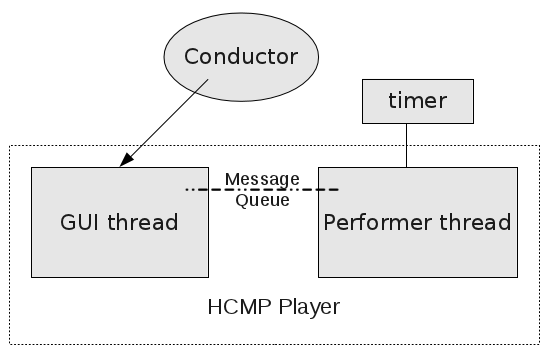
\includegraphics[width=0.65\linewidth]{2/2.png}}
\caption{Architecture of the HCMP Midi Player}
\label{fig:speciation}
\end{figure}

Internally, the Player will have two threads, with one thread for
GUI interactive control (GUI thread) and the other thread for 
performing music data (performer thread). 
The two threads will communicate with each other through a shared 
message queue, we can assume the message 
queue is large enough to avoid blocks for both caller and callee threads. 
The performaner thread
will handle time critical operations, and there will be a timer setup 
before this thread is created. The goal of the timer is to 
wake up the performer thread periodically. Everytime the performer 
thread's timer callback function is invoked, 
it will check the message queue and process any command from the control thread.
Figure 2 illustrates the overall structure of the Player.

%Most organisms use polymers of glucose units for energy storage and differ only slightly in the way they link together monomers to sometimes gigantic macromolecules. Dextran of bacteria is made from long chains of $\alpha$-1,6-linked glucose units. 

%: ----------------------- HELP: special characters
% above you can see how special characters are coded; e.g. $\alpha$
% below are the most frequently used codes:
%$\alpha$  $\beta$  $\gamma$  $\delta$

%$^{chars to be superscripted}$  OR $^x$ (for a single character)
%$_{chars to be suberscripted}$  OR $_x$

%>  $>$  greater,  <  $<$  less
%≥  $\ge$  greater than or equal, ≤  $\ge$  lesser than or equal
%~  $\sim$  similar to

%$^{\circ}$C   ° as in degree C
%±  \pm     plus/minus sign

%$\AA$     produces  Å (Angstrom)

% dextran, starch, glycogen continued
%Starch of plants and glycogen of animals consists of $\alpha$-1,4-glycosidic glucose polymers \cite{lastname07}. See figure \ref{largepotato} for a comparison of glucose polymer structure and chemistry. 

%Two references can be placed separated by a comma \cite{lastname07,name06}.

%: ----------------------- HELP: references
% References can be links to figures, tables, sections, or references.
% For figures, tables, and text you define the target of the link with \label{XYZ}. Then you call cross-link with the command \ref{XYZ}, as above
% Citations are bound in a very similar way with \cite{XYZ}. You store your references in a BibTex file with a programme like BibDesk.



%\figuremacro{largepotato}{A common glucose polymers}{The figure shows starch granules in potato cells, taken from \href{http://molecularexpressions.com/micro/gallery/burgersnfries/burgersnfries4.html}{Molecular Expressions}.}

%: ----------------------- HELP: adding figures with macros
% This template provides a very convenient way to add figures with minimal code.
% \figuremacro{1}{2}{3}{4} calls up a series of commands formating your image.
% 1 = name of the file without extension; PNG, JPEG is ok; GIF doesn't work
% 2 = title of the figure AND the name of the label for cross-linking
% 3 = caption text for the figure

%: ----------------------- HELP: www links
% You can also see above how, www links are placed
% \href{http://www.something.net}{link text}

%\figuremacroW{largepotato}{Title}{Caption}{0.8}

% variation of the above macro with a width setting
% \figuremacroW{1}{2}{3}{4}
% 1-3 as above
% 4 = size relative to text width which is 1; use this to reduce figures


%Insulin stimulates the following processes:
%
%\begin{itemize}
%\item muscle and fat cells remove glucose from the blood,
%\item cells breakdown glucose via glycolysis and the citrate cycle, storing its energy in the form of ATP,
%\item liver and muscle store glucose as glycogen as a short-term energy reserve,
%\item adipose tissue stores glucose as fat for long-term energy reserve, and
%\item cells use glucose for protein synthesis.
%\end{itemize}

%: ----------------------- HELP: lists
% This is how you generate lists in LaTeX.
% If you replace {itemize} by {enumerate} you get a numbered list.

%: ----------------------- HELP: tables
% Directly coding tables in latex is tiresome. See below.
% I would recommend using a converter macro that allows you to make the table in Excel and convert them into latex code which you can then paste into your doc.
% This is the link: http://www.softpedia.com/get/Office-tools/Other-Office-Tools/Excel2Latex.shtml
% It's a Excel template file containing a macro for the conversion.

% There you go. You already know the most important things.
			
\chapter{Introduction}

% the code below specifies where the figures are stored
\ifpdf
    \graphicspath{{1_introduction/figures/PNG/}{1_introduction/figures/PDF/}{1_introduction/figures/}}
\else
    \graphicspath{{1_introduction/figures/EPS/}{1_introduction/figures/}}
\fi

\section{Overview}
Computers have been widely used in music performances for many years. Some
advanced systems use the computer as a independent module to replace a
single instrument in an orchestra. In popular music computers have proved
to be particularly successful. Both classical and popular music have many
opportunities for innovative applications used by highly intelligent and
coordinated computer music systems. With more powerful algorithms and more
advanced sensing devices, computer music systems have the potential to
replace musicians. In the future, computer music systems will inspire new 
musical directions based on new
capabilities and generate new concepts from new technologies.

Live popular music offers a wealth of opportunities for computing and music
research.  We term the integration of computers as independent autonomous
performers into popular live music performances as Human Computer Music
Performance (HCMP). In HCMP computers become more than instruments and are,
in some degree, seen as performers. To bring HCMP into the realm of popular
music performance, certain problems need to be solved. 

One problem is that
popular music is organized around a tight synchronization to beats and a
computer cannot reliably and efficiently adapt to human tempo variations.
Another significant problem is that an HCMP project is a large complex
system which contain many components, each one relying on the cooperation of several
different subcomponents to complete its task.

The motivation behind the HCMP Player is to provide a good solution to these
problems. When successful, the HCMP Player will display different
representations of music, work as an accompaniment  and quickly adjust its
tempo to follow the performer. A clearly defined programming interface is
also required in order to foster communication and cooperation with all
components within the system. To create such a player, we must coordinate
time between different media. We need at least two functional components,
one component working as ``backend'' and responsible for coordinating and
scheduling different music events, the other, working as ``frontend'', will
receive commands from the user or other components and dynamically adjust
play sequence and tempo based on those requests.

This paper begins with the role of the HCMP Player in the HCMP project. Then
the ``big picture of'' of the HCMP project will be discussed, followed by a
presentation of the individual HCMP components. Finally the question that how
does the HMCP Player fit into the whole picture will be addressed. In the
following three chapters design issues with the HCMP Player are addressed.
Each chapter approaches the problem from a different perspective. Chapter 2
describes the design of Graphic User Interface (GUI) of HCMP Player together
with a detailed explanation of all the GUI components' usage and function.
Chapter 3 describes the ``backend'' of the HCMP Player - the player engine,
and illustrates how the player engine cooperates and communicates with the
GUI to complete external requests. Chapter 4 addresses the network
communication problem between multiple players. A set of unified API is
defined to make the HCMP Player compatible with other components in the HCMP
project.  Chapter 5 describes the implementation details of the HCMP Player
and includes pseucode to provide a clear explanation of this. Chapter 6
focuses on the evaluation of the HCMP Player, a full list of feature points
will be given and a clear success criteria used to evaluate the HCMP Player
will be defined.  In chapter 7, I summarize my work and propose possible
future works.

\section{Background}

Before making a formal introduction to the background of HCMP Player. 
I would like to make short review of  
some existed human computer music systems. The most common use of computer in
music performance is through computer instruments, typically keyboards.
These, and other electronic instruments, are essentially substitutes for traditional
instruments and rely upon human musicians for their control and coordination with
other musicians. Many composers of interactive contemporary art music use computers
to generate music in real time, often in response to live performers.

Another meaningful use of computer in music is computer accompaniment system 
\cite{Roger:89}, 
whcih solves the synchronization problem by assuming a pre-determined 
score (music notation). During the performance, a performer expressively 
played music score, while the accompaniment system ``listen'' and analysis, 
then follows the performer 
in the score and synchronizes an accompaniment.

In live popular music peformance, computer is quite useful too.
The computer has had a significant
impact on popular music through drum machines, sequencers and loop-based
interfaces, but one can argue that popular music has adapted to new technology
rather than the other way around. The sound and beat of drum machines seems stiff,
mechanical, and monotonous to many musicians, but that became the trance-like
foundation of club dance music and other forms . Similarly, 
the inability of
sequencers and other beat-based software to “listen” to human musicians has led to
performances with click tracks in fixed media or simply a fixed drum track that live
musicians must follow. Ableton Live \cite{Ableton:2011} is an example of software that
uses a beat, measure, and section framework to synchronize music in live
performance, but the program is not well suited to adapting to the tempo of live
musicians. Robertson and Plumbley \cite{Robertson:2007} used a real-time beat 
tracker in
conjunction with Ableton Live software to synchronize pre-recorded music 
to a live drummer. This extension could be considered HCMP.
The table 1.1 summarize some of existed computer music systems and their usage.

\begin{table}[htdp]
\centering
\begin{tabular}{| p{5cm} | p{8cm} |} % ccc means 3 columns, all centered; alternatives are l, r

\hline
Computer Instruments & Direct physical interaction with virtual instruments \\

\hline 
Interactive Contemporary Art Music & Composed interactions; often unconstrained by
traditional harmony or rhythm.\\

\hline
Computer Accompaniment & score following synchronizes computer to live performer.\\

\hline
Fixed Media  & Many musical styles and formats. Live performers
synchronize to fixed recording.\\

\hline
Conducting System & Synchronize live computer performance by tapping or
gesturing beats. Best with “expressive”
traditional/classical music.\\
\hline
\end{tabular}
\caption[Computer Music Systems Summary]{Computer Music Systems Summary}
\label{latexin_genes} % label for cross-links with \ref{latexin_genes}
\end{table}

\section{Objective}
The objective of HCMP \cite{Dawen:2011} is to create an autonomous 
``artificial performer'' with the ability of a human-level musical performance. 
Hopefully, HCMP does not require a human operator's interfere, the system itself 
is designed to be adaptive and responsive. With sophisticated listening and sensing
component, HCMP is able to adjust related system parameters in real-time during 
performance. From functional perspective, we can divide HCMP into two main
categories: music preparation and music performance. Music preparation
part aims to work and understand with multiple music representations. Music
performance part is to deal with various issues regarding to question 
how to play music.     

An important component of the music performance part is the HCMP Player, 
which is able to flexibly  
adjust and respond to changes of music signal. Figure 1 illustrates relationship 
between scheduler, conductor and HCMP Plyaer. During performance, the HCMP Player will 
be controlled by conductor and constantly receive control messages 
from its conductor. In this project, I will design, implement the HCMP midi player 
for the HCMP project that is able to fully cooperate with conductor and scheduler.
\begin{figure}[H] % Example image
\center{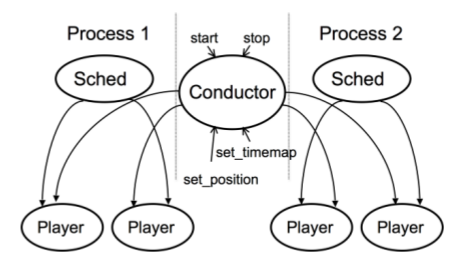
\includegraphics[width=0.65\linewidth]{1/1.png}}
\caption{Key Components of HCMP}
\label{fig:speciation}
\end{figure}
 

\section{Architecture}
\subsection{HCMP Architecture}
Figure 1.2 shows architecture of the whole HCMP project. it mainly contain 5 
subsystems. A brief description of each subsystem and its function will be
given in following paragraphs.
\begin{figure}[H] % Example image
\center{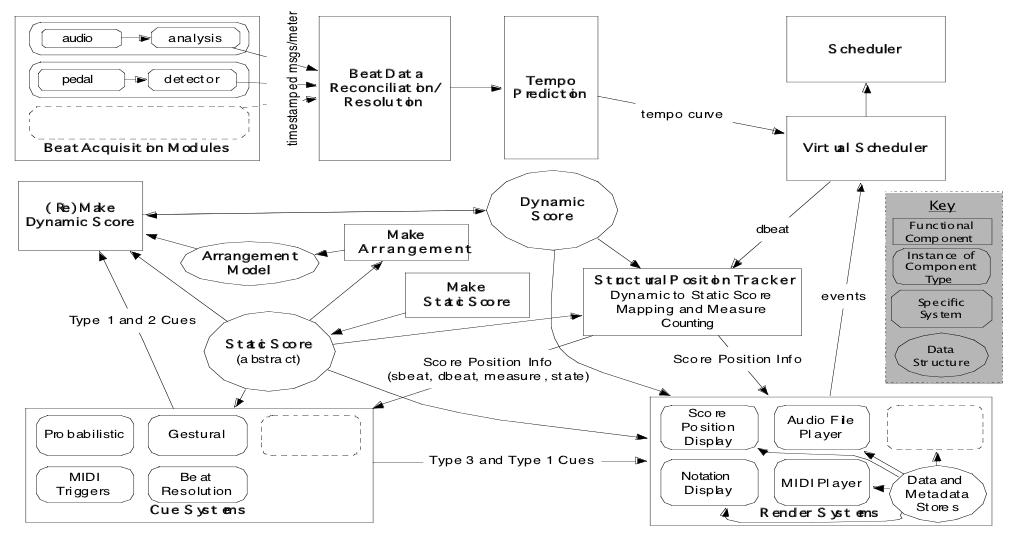
\includegraphics[width=1\linewidth]{1/2.png}}
\caption{Whole Picture of the HCMP Project}
\label{fig:speciation}
\end{figure}

\subsubsection{Real-Time System}
Real-time components are needed to keep an HCMP system coordinated with
the human musicians in an ensemble. Real-time synchronization aspects are
handled by components such as beat and tempo tracking systems.

\subsubsection{Abstract-Time System}
Abstract time components are needed to manage and schedule score events in
the context of the performance. The virtual scheduler and its associated systems are
concerned with the abstract time aspects of the system. The virtual scheduler should
reschedule events scheduled on a nominal time trajectory by warping the event times
according to the incoming tempo data from the tempo prediction system. Events are
then passed to an actual scheduler for real-time scheduling.

\subsubsection{Score and Arrangement System}
Score management is handled by the functional components in the center box of
the diagram. These systems will allow a human musician to encode, manage, and
arrange scores for performance.

\subsubsection{Cueing System}
Cueing systems are required to allow the computer system to react to high-level
structural and synchronization changes during performance (e.g. additional
repetitions of a chorus). There are mainly three types of cues:
\begin{enumerate}
  \item Static Score Position Cue. This cue is necessary when synchronization with the
static score is lost. Issuing it will cause the dynamic score to be re-made
accordingly.
  \item Intention Cue. This cue is needed to inform the computer of the intended
direction of the current performance (e.g. exiting a vamp section or adding an
additional chorus). Issuing it (e.g. using a MIDI trigger, gesture recognition or
other method) will cause the future dynamic score to be remade.
  \item Voicing/Arrangement Cue. This cue is needed to allow control over the voicing
of a section (e.g. it may be desirable to prevent a particular instrumental group
from playing on the first time through a repeat but allow them to play on the
second). Issuing this type of cue affects only the render system to which it is
issued.
\end{enumerate}

\subsubsection{Render System}
Render systems are responsible for providing different kindos multi-media output 
at the appropriate time. Render system will be designed as some kind of ``add-on'' 
for the HCMP, so that we could flexibly change, remove and update the render system.
With unified programming interface, each reander system is provided similar raw 
data and each system should also define its own way of parsing the raw data.
Sometimes, metadata is required to link these data elements to their appropriate 
static score position (and thus to
their appropriate scheduling as the dynamic score is played). A standardized
format will be required for this to relate static-score measure-numbers and the
dynamic score position and context to the properties of the format concerned. This
provide render systems more flexibility to determine how they need to deal with 
beat-level information or simply use the measure-level data, for example, a score 
display system might map a measure to image information or an audio render 
system might represent audio at the beat level.

%Abstract beat-time information can thus be linked to real-time source material
%(to allow the correct scheduling of real-time data) while allowing the overall system
%to remain oblivious to the specific source formats being used. Render systems
%should use a callback interface whereby they schedule events with the scheduling
%systems. These call the appropriate renderer at the scheduled time, causing
%synchronized real-time output of media in accordance with the dynamic score and
%beat tracking information.

\subsection{HCMP Player Architecture}
From system architectures' perspective, the interal HCMP Player is mainly made up of
two threads, we name the thread that taking
care of user input, maintaining graphic state GUI thread. And the thread worked as   
player engine is called performer thread, each thread is a independent 
module and executed in a separated thread space. Timer will be external source 
which periodically invoke the user in do some task. A timer usually come with a 
language library, so its implementation is within the category of this paper.

During the performance, the HCMP Player will act as 
the server for the conductor component, which is constantly 
receiving control messages and responding accordingly. 

\begin{figure}[H]
\center{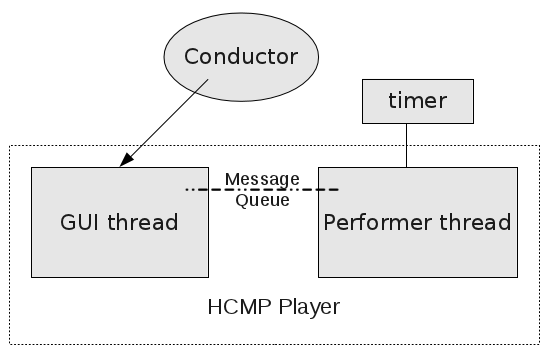
\includegraphics[width=0.65\linewidth]{2/2.png}}
\caption{Architecture of the HCMP Midi Player}
\label{fig:speciation}
\end{figure}

Internally, the Player will have two threads, with one thread for
GUI interactive control (GUI thread) and the other thread for 
performing music data (performer thread). 
The two threads will communicate with each other through a shared 
message queue, we can assume the message 
queue is large enough to avoid blocks for both caller and callee threads. 
The performaner thread
will handle time critical operations, and there will be a timer setup 
before this thread is created. The goal of the timer is to 
wake up the performer thread periodically. Everytime the performer 
thread's timer callback function is invoked, 
it will check the message queue and process any command from the control thread.
Figure 2 illustrates the overall structure of the Player.

%Most organisms use polymers of glucose units for energy storage and differ only slightly in the way they link together monomers to sometimes gigantic macromolecules. Dextran of bacteria is made from long chains of $\alpha$-1,6-linked glucose units. 

%: ----------------------- HELP: special characters
% above you can see how special characters are coded; e.g. $\alpha$
% below are the most frequently used codes:
%$\alpha$  $\beta$  $\gamma$  $\delta$

%$^{chars to be superscripted}$  OR $^x$ (for a single character)
%$_{chars to be suberscripted}$  OR $_x$

%>  $>$  greater,  <  $<$  less
%≥  $\ge$  greater than or equal, ≤  $\ge$  lesser than or equal
%~  $\sim$  similar to

%$^{\circ}$C   ° as in degree C
%±  \pm     plus/minus sign

%$\AA$     produces  Å (Angstrom)

% dextran, starch, glycogen continued
%Starch of plants and glycogen of animals consists of $\alpha$-1,4-glycosidic glucose polymers \cite{lastname07}. See figure \ref{largepotato} for a comparison of glucose polymer structure and chemistry. 

%Two references can be placed separated by a comma \cite{lastname07,name06}.

%: ----------------------- HELP: references
% References can be links to figures, tables, sections, or references.
% For figures, tables, and text you define the target of the link with \label{XYZ}. Then you call cross-link with the command \ref{XYZ}, as above
% Citations are bound in a very similar way with \cite{XYZ}. You store your references in a BibTex file with a programme like BibDesk.



%\figuremacro{largepotato}{A common glucose polymers}{The figure shows starch granules in potato cells, taken from \href{http://molecularexpressions.com/micro/gallery/burgersnfries/burgersnfries4.html}{Molecular Expressions}.}

%: ----------------------- HELP: adding figures with macros
% This template provides a very convenient way to add figures with minimal code.
% \figuremacro{1}{2}{3}{4} calls up a series of commands formating your image.
% 1 = name of the file without extension; PNG, JPEG is ok; GIF doesn't work
% 2 = title of the figure AND the name of the label for cross-linking
% 3 = caption text for the figure

%: ----------------------- HELP: www links
% You can also see above how, www links are placed
% \href{http://www.something.net}{link text}

%\figuremacroW{largepotato}{Title}{Caption}{0.8}

% variation of the above macro with a width setting
% \figuremacroW{1}{2}{3}{4}
% 1-3 as above
% 4 = size relative to text width which is 1; use this to reduce figures


%Insulin stimulates the following processes:
%
%\begin{itemize}
%\item muscle and fat cells remove glucose from the blood,
%\item cells breakdown glucose via glycolysis and the citrate cycle, storing its energy in the form of ATP,
%\item liver and muscle store glucose as glycogen as a short-term energy reserve,
%\item adipose tissue stores glucose as fat for long-term energy reserve, and
%\item cells use glucose for protein synthesis.
%\end{itemize}

%: ----------------------- HELP: lists
% This is how you generate lists in LaTeX.
% If you replace {itemize} by {enumerate} you get a numbered list.

%: ----------------------- HELP: tables
% Directly coding tables in latex is tiresome. See below.
% I would recommend using a converter macro that allows you to make the table in Excel and convert them into latex code which you can then paste into your doc.
% This is the link: http://www.softpedia.com/get/Office-tools/Other-Office-Tools/Excel2Latex.shtml
% It's a Excel template file containing a macro for the conversion.

% There you go. You already know the most important things.
	
%\chapter{Introduction}

% the code below specifies where the figures are stored
\ifpdf
    \graphicspath{{1_introduction/figures/PNG/}{1_introduction/figures/PDF/}{1_introduction/figures/}}
\else
    \graphicspath{{1_introduction/figures/EPS/}{1_introduction/figures/}}
\fi

\section{Overview}
Computers have been widely used in music performances for many years. Some
advanced systems use the computer as a independent module to replace a
single instrument in an orchestra. In popular music computers have proved
to be particularly successful. Both classical and popular music have many
opportunities for innovative applications used by highly intelligent and
coordinated computer music systems. With more powerful algorithms and more
advanced sensing devices, computer music systems have the potential to
replace musicians. In the future, computer music systems will inspire new 
musical directions based on new
capabilities and generate new concepts from new technologies.

Live popular music offers a wealth of opportunities for computing and music
research.  We term the integration of computers as independent autonomous
performers into popular live music performances as Human Computer Music
Performance (HCMP). In HCMP computers become more than instruments and are,
in some degree, seen as performers. To bring HCMP into the realm of popular
music performance, certain problems need to be solved. 

One problem is that
popular music is organized around a tight synchronization to beats and a
computer cannot reliably and efficiently adapt to human tempo variations.
Another significant problem is that an HCMP project is a large complex
system which contain many components, each one relying on the cooperation of several
different subcomponents to complete its task.

The motivation behind the HCMP Player is to provide a good solution to these
problems. When successful, the HCMP Player will display different
representations of music, work as an accompaniment  and quickly adjust its
tempo to follow the performer. A clearly defined programming interface is
also required in order to foster communication and cooperation with all
components within the system. To create such a player, we must coordinate
time between different media. We need at least two functional components,
one component working as ``backend'' and responsible for coordinating and
scheduling different music events, the other, working as ``frontend'', will
receive commands from the user or other components and dynamically adjust
play sequence and tempo based on those requests.

This paper begins with the role of the HCMP Player in the HCMP project. Then
the ``big picture of'' of the HCMP project will be discussed, followed by a
presentation of the individual HCMP components. Finally the question that how
does the HMCP Player fit into the whole picture will be addressed. In the
following three chapters design issues with the HCMP Player are addressed.
Each chapter approaches the problem from a different perspective. Chapter 2
describes the design of Graphic User Interface (GUI) of HCMP Player together
with a detailed explanation of all the GUI components' usage and function.
Chapter 3 describes the ``backend'' of the HCMP Player - the player engine,
and illustrates how the player engine cooperates and communicates with the
GUI to complete external requests. Chapter 4 addresses the network
communication problem between multiple players. A set of unified API is
defined to make the HCMP Player compatible with other components in the HCMP
project.  Chapter 5 describes the implementation details of the HCMP Player
and includes pseucode to provide a clear explanation of this. Chapter 6
focuses on the evaluation of the HCMP Player, a full list of feature points
will be given and a clear success criteria used to evaluate the HCMP Player
will be defined.  In chapter 7, I summarize my work and propose possible
future works.

\section{Background}

Before making a formal introduction to the background of HCMP Player. 
I would like to make short review of  
some existed human computer music systems. The most common use of computer in
music performance is through computer instruments, typically keyboards.
These, and other electronic instruments, are essentially substitutes for traditional
instruments and rely upon human musicians for their control and coordination with
other musicians. Many composers of interactive contemporary art music use computers
to generate music in real time, often in response to live performers.

Another meaningful use of computer in music is computer accompaniment system 
\cite{Roger:89}, 
whcih solves the synchronization problem by assuming a pre-determined 
score (music notation). During the performance, a performer expressively 
played music score, while the accompaniment system ``listen'' and analysis, 
then follows the performer 
in the score and synchronizes an accompaniment.

In live popular music peformance, computer is quite useful too.
The computer has had a significant
impact on popular music through drum machines, sequencers and loop-based
interfaces, but one can argue that popular music has adapted to new technology
rather than the other way around. The sound and beat of drum machines seems stiff,
mechanical, and monotonous to many musicians, but that became the trance-like
foundation of club dance music and other forms . Similarly, 
the inability of
sequencers and other beat-based software to “listen” to human musicians has led to
performances with click tracks in fixed media or simply a fixed drum track that live
musicians must follow. Ableton Live \cite{Ableton:2011} is an example of software that
uses a beat, measure, and section framework to synchronize music in live
performance, but the program is not well suited to adapting to the tempo of live
musicians. Robertson and Plumbley \cite{Robertson:2007} used a real-time beat 
tracker in
conjunction with Ableton Live software to synchronize pre-recorded music 
to a live drummer. This extension could be considered HCMP.
The table 1.1 summarize some of existed computer music systems and their usage.

\begin{table}[htdp]
\centering
\begin{tabular}{| p{5cm} | p{8cm} |} % ccc means 3 columns, all centered; alternatives are l, r

\hline
Computer Instruments & Direct physical interaction with virtual instruments \\

\hline 
Interactive Contemporary Art Music & Composed interactions; often unconstrained by
traditional harmony or rhythm.\\

\hline
Computer Accompaniment & score following synchronizes computer to live performer.\\

\hline
Fixed Media  & Many musical styles and formats. Live performers
synchronize to fixed recording.\\

\hline
Conducting System & Synchronize live computer performance by tapping or
gesturing beats. Best with “expressive”
traditional/classical music.\\
\hline
\end{tabular}
\caption[Computer Music Systems Summary]{Computer Music Systems Summary}
\label{latexin_genes} % label for cross-links with \ref{latexin_genes}
\end{table}

\section{Objective}
The objective of HCMP \cite{Dawen:2011} is to create an autonomous 
``artificial performer'' with the ability of a human-level musical performance. 
Hopefully, HCMP does not require a human operator's interfere, the system itself 
is designed to be adaptive and responsive. With sophisticated listening and sensing
component, HCMP is able to adjust related system parameters in real-time during 
performance. From functional perspective, we can divide HCMP into two main
categories: music preparation and music performance. Music preparation
part aims to work and understand with multiple music representations. Music
performance part is to deal with various issues regarding to question 
how to play music.     

An important component of the music performance part is the HCMP Player, 
which is able to flexibly  
adjust and respond to changes of music signal. Figure 1 illustrates relationship 
between scheduler, conductor and HCMP Plyaer. During performance, the HCMP Player will 
be controlled by conductor and constantly receive control messages 
from its conductor. In this project, I will design, implement the HCMP midi player 
for the HCMP project that is able to fully cooperate with conductor and scheduler.
\begin{figure}[H] % Example image
\center{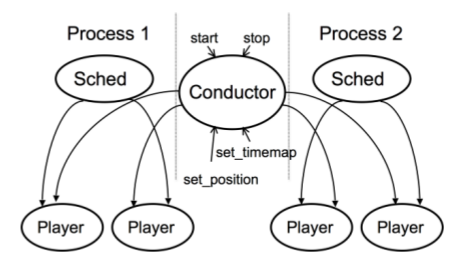
\includegraphics[width=0.65\linewidth]{1/1.png}}
\caption{Key Components of HCMP}
\label{fig:speciation}
\end{figure}
 

\section{Architecture}
\subsection{HCMP Architecture}
Figure 1.2 shows architecture of the whole HCMP project. it mainly contain 5 
subsystems. A brief description of each subsystem and its function will be
given in following paragraphs.
\begin{figure}[H] % Example image
\center{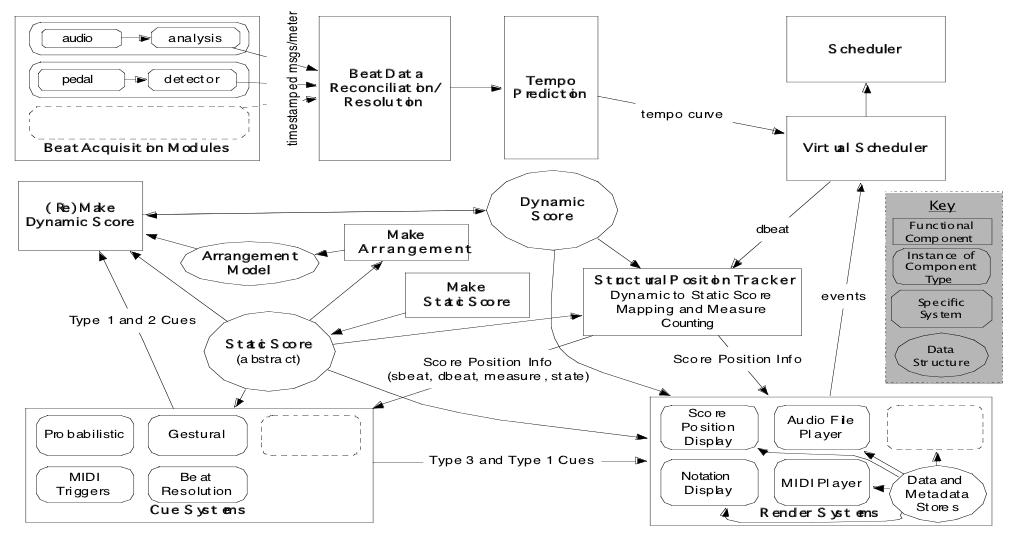
\includegraphics[width=1\linewidth]{1/2.png}}
\caption{Whole Picture of the HCMP Project}
\label{fig:speciation}
\end{figure}

\subsubsection{Real-Time System}
Real-time components are needed to keep an HCMP system coordinated with
the human musicians in an ensemble. Real-time synchronization aspects are
handled by components such as beat and tempo tracking systems.

\subsubsection{Abstract-Time System}
Abstract time components are needed to manage and schedule score events in
the context of the performance. The virtual scheduler and its associated systems are
concerned with the abstract time aspects of the system. The virtual scheduler should
reschedule events scheduled on a nominal time trajectory by warping the event times
according to the incoming tempo data from the tempo prediction system. Events are
then passed to an actual scheduler for real-time scheduling.

\subsubsection{Score and Arrangement System}
Score management is handled by the functional components in the center box of
the diagram. These systems will allow a human musician to encode, manage, and
arrange scores for performance.

\subsubsection{Cueing System}
Cueing systems are required to allow the computer system to react to high-level
structural and synchronization changes during performance (e.g. additional
repetitions of a chorus). There are mainly three types of cues:
\begin{enumerate}
  \item Static Score Position Cue. This cue is necessary when synchronization with the
static score is lost. Issuing it will cause the dynamic score to be re-made
accordingly.
  \item Intention Cue. This cue is needed to inform the computer of the intended
direction of the current performance (e.g. exiting a vamp section or adding an
additional chorus). Issuing it (e.g. using a MIDI trigger, gesture recognition or
other method) will cause the future dynamic score to be remade.
  \item Voicing/Arrangement Cue. This cue is needed to allow control over the voicing
of a section (e.g. it may be desirable to prevent a particular instrumental group
from playing on the first time through a repeat but allow them to play on the
second). Issuing this type of cue affects only the render system to which it is
issued.
\end{enumerate}

\subsubsection{Render System}
Render systems are responsible for providing different kindos multi-media output 
at the appropriate time. Render system will be designed as some kind of ``add-on'' 
for the HCMP, so that we could flexibly change, remove and update the render system.
With unified programming interface, each reander system is provided similar raw 
data and each system should also define its own way of parsing the raw data.
Sometimes, metadata is required to link these data elements to their appropriate 
static score position (and thus to
their appropriate scheduling as the dynamic score is played). A standardized
format will be required for this to relate static-score measure-numbers and the
dynamic score position and context to the properties of the format concerned. This
provide render systems more flexibility to determine how they need to deal with 
beat-level information or simply use the measure-level data, for example, a score 
display system might map a measure to image information or an audio render 
system might represent audio at the beat level.

%Abstract beat-time information can thus be linked to real-time source material
%(to allow the correct scheduling of real-time data) while allowing the overall system
%to remain oblivious to the specific source formats being used. Render systems
%should use a callback interface whereby they schedule events with the scheduling
%systems. These call the appropriate renderer at the scheduled time, causing
%synchronized real-time output of media in accordance with the dynamic score and
%beat tracking information.

\subsection{HCMP Player Architecture}
From system architectures' perspective, the interal HCMP Player is mainly made up of
two threads, we name the thread that taking
care of user input, maintaining graphic state GUI thread. And the thread worked as   
player engine is called performer thread, each thread is a independent 
module and executed in a separated thread space. Timer will be external source 
which periodically invoke the user in do some task. A timer usually come with a 
language library, so its implementation is within the category of this paper.

During the performance, the HCMP Player will act as 
the server for the conductor component, which is constantly 
receiving control messages and responding accordingly. 

\begin{figure}[H]
\center{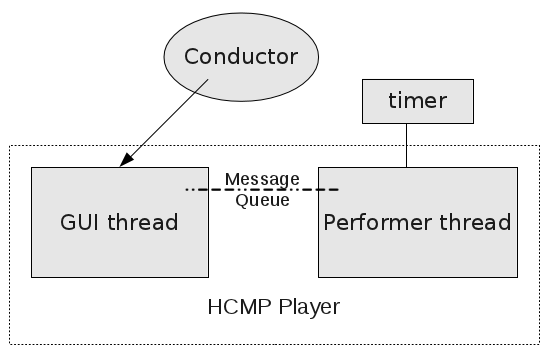
\includegraphics[width=0.65\linewidth]{2/2.png}}
\caption{Architecture of the HCMP Midi Player}
\label{fig:speciation}
\end{figure}

Internally, the Player will have two threads, with one thread for
GUI interactive control (GUI thread) and the other thread for 
performing music data (performer thread). 
The two threads will communicate with each other through a shared 
message queue, we can assume the message 
queue is large enough to avoid blocks for both caller and callee threads. 
The performaner thread
will handle time critical operations, and there will be a timer setup 
before this thread is created. The goal of the timer is to 
wake up the performer thread periodically. Everytime the performer 
thread's timer callback function is invoked, 
it will check the message queue and process any command from the control thread.
Figure 2 illustrates the overall structure of the Player.

%Most organisms use polymers of glucose units for energy storage and differ only slightly in the way they link together monomers to sometimes gigantic macromolecules. Dextran of bacteria is made from long chains of $\alpha$-1,6-linked glucose units. 

%: ----------------------- HELP: special characters
% above you can see how special characters are coded; e.g. $\alpha$
% below are the most frequently used codes:
%$\alpha$  $\beta$  $\gamma$  $\delta$

%$^{chars to be superscripted}$  OR $^x$ (for a single character)
%$_{chars to be suberscripted}$  OR $_x$

%>  $>$  greater,  <  $<$  less
%≥  $\ge$  greater than or equal, ≤  $\ge$  lesser than or equal
%~  $\sim$  similar to

%$^{\circ}$C   ° as in degree C
%±  \pm     plus/minus sign

%$\AA$     produces  Å (Angstrom)

% dextran, starch, glycogen continued
%Starch of plants and glycogen of animals consists of $\alpha$-1,4-glycosidic glucose polymers \cite{lastname07}. See figure \ref{largepotato} for a comparison of glucose polymer structure and chemistry. 

%Two references can be placed separated by a comma \cite{lastname07,name06}.

%: ----------------------- HELP: references
% References can be links to figures, tables, sections, or references.
% For figures, tables, and text you define the target of the link with \label{XYZ}. Then you call cross-link with the command \ref{XYZ}, as above
% Citations are bound in a very similar way with \cite{XYZ}. You store your references in a BibTex file with a programme like BibDesk.



%\figuremacro{largepotato}{A common glucose polymers}{The figure shows starch granules in potato cells, taken from \href{http://molecularexpressions.com/micro/gallery/burgersnfries/burgersnfries4.html}{Molecular Expressions}.}

%: ----------------------- HELP: adding figures with macros
% This template provides a very convenient way to add figures with minimal code.
% \figuremacro{1}{2}{3}{4} calls up a series of commands formating your image.
% 1 = name of the file without extension; PNG, JPEG is ok; GIF doesn't work
% 2 = title of the figure AND the name of the label for cross-linking
% 3 = caption text for the figure

%: ----------------------- HELP: www links
% You can also see above how, www links are placed
% \href{http://www.something.net}{link text}

%\figuremacroW{largepotato}{Title}{Caption}{0.8}

% variation of the above macro with a width setting
% \figuremacroW{1}{2}{3}{4}
% 1-3 as above
% 4 = size relative to text width which is 1; use this to reduce figures


%Insulin stimulates the following processes:
%
%\begin{itemize}
%\item muscle and fat cells remove glucose from the blood,
%\item cells breakdown glucose via glycolysis and the citrate cycle, storing its energy in the form of ATP,
%\item liver and muscle store glucose as glycogen as a short-term energy reserve,
%\item adipose tissue stores glucose as fat for long-term energy reserve, and
%\item cells use glucose for protein synthesis.
%\end{itemize}

%: ----------------------- HELP: lists
% This is how you generate lists in LaTeX.
% If you replace {itemize} by {enumerate} you get a numbered list.

%: ----------------------- HELP: tables
% Directly coding tables in latex is tiresome. See below.
% I would recommend using a converter macro that allows you to make the table in Excel and convert them into latex code which you can then paste into your doc.
% This is the link: http://www.softpedia.com/get/Office-tools/Other-Office-Tools/Excel2Latex.shtml
% It's a Excel template file containing a macro for the conversion.

% There you go. You already know the most important things.

\chapter{Introduction}

% the code below specifies where the figures are stored
\ifpdf
    \graphicspath{{1_introduction/figures/PNG/}{1_introduction/figures/PDF/}{1_introduction/figures/}}
\else
    \graphicspath{{1_introduction/figures/EPS/}{1_introduction/figures/}}
\fi

\section{Overview}
Computers have been widely used in music performances for many years. Some
advanced systems use the computer as a independent module to replace a
single instrument in an orchestra. In popular music computers have proved
to be particularly successful. Both classical and popular music have many
opportunities for innovative applications used by highly intelligent and
coordinated computer music systems. With more powerful algorithms and more
advanced sensing devices, computer music systems have the potential to
replace musicians. In the future, computer music systems will inspire new 
musical directions based on new
capabilities and generate new concepts from new technologies.

Live popular music offers a wealth of opportunities for computing and music
research.  We term the integration of computers as independent autonomous
performers into popular live music performances as Human Computer Music
Performance (HCMP). In HCMP computers become more than instruments and are,
in some degree, seen as performers. To bring HCMP into the realm of popular
music performance, certain problems need to be solved. 

One problem is that
popular music is organized around a tight synchronization to beats and a
computer cannot reliably and efficiently adapt to human tempo variations.
Another significant problem is that an HCMP project is a large complex
system which contain many components, each one relying on the cooperation of several
different subcomponents to complete its task.

The motivation behind the HCMP Player is to provide a good solution to these
problems. When successful, the HCMP Player will display different
representations of music, work as an accompaniment  and quickly adjust its
tempo to follow the performer. A clearly defined programming interface is
also required in order to foster communication and cooperation with all
components within the system. To create such a player, we must coordinate
time between different media. We need at least two functional components,
one component working as ``backend'' and responsible for coordinating and
scheduling different music events, the other, working as ``frontend'', will
receive commands from the user or other components and dynamically adjust
play sequence and tempo based on those requests.

This paper begins with the role of the HCMP Player in the HCMP project. Then
the ``big picture of'' of the HCMP project will be discussed, followed by a
presentation of the individual HCMP components. Finally the question that how
does the HMCP Player fit into the whole picture will be addressed. In the
following three chapters design issues with the HCMP Player are addressed.
Each chapter approaches the problem from a different perspective. Chapter 2
describes the design of Graphic User Interface (GUI) of HCMP Player together
with a detailed explanation of all the GUI components' usage and function.
Chapter 3 describes the ``backend'' of the HCMP Player - the player engine,
and illustrates how the player engine cooperates and communicates with the
GUI to complete external requests. Chapter 4 addresses the network
communication problem between multiple players. A set of unified API is
defined to make the HCMP Player compatible with other components in the HCMP
project.  Chapter 5 describes the implementation details of the HCMP Player
and includes pseucode to provide a clear explanation of this. Chapter 6
focuses on the evaluation of the HCMP Player, a full list of feature points
will be given and a clear success criteria used to evaluate the HCMP Player
will be defined.  In chapter 7, I summarize my work and propose possible
future works.

\section{Background}

Before making a formal introduction to the background of HCMP Player. 
I would like to make short review of  
some existed human computer music systems. The most common use of computer in
music performance is through computer instruments, typically keyboards.
These, and other electronic instruments, are essentially substitutes for traditional
instruments and rely upon human musicians for their control and coordination with
other musicians. Many composers of interactive contemporary art music use computers
to generate music in real time, often in response to live performers.

Another meaningful use of computer in music is computer accompaniment system 
\cite{Roger:89}, 
whcih solves the synchronization problem by assuming a pre-determined 
score (music notation). During the performance, a performer expressively 
played music score, while the accompaniment system ``listen'' and analysis, 
then follows the performer 
in the score and synchronizes an accompaniment.

In live popular music peformance, computer is quite useful too.
The computer has had a significant
impact on popular music through drum machines, sequencers and loop-based
interfaces, but one can argue that popular music has adapted to new technology
rather than the other way around. The sound and beat of drum machines seems stiff,
mechanical, and monotonous to many musicians, but that became the trance-like
foundation of club dance music and other forms . Similarly, 
the inability of
sequencers and other beat-based software to “listen” to human musicians has led to
performances with click tracks in fixed media or simply a fixed drum track that live
musicians must follow. Ableton Live \cite{Ableton:2011} is an example of software that
uses a beat, measure, and section framework to synchronize music in live
performance, but the program is not well suited to adapting to the tempo of live
musicians. Robertson and Plumbley \cite{Robertson:2007} used a real-time beat 
tracker in
conjunction with Ableton Live software to synchronize pre-recorded music 
to a live drummer. This extension could be considered HCMP.
The table 1.1 summarize some of existed computer music systems and their usage.

\begin{table}[htdp]
\centering
\begin{tabular}{| p{5cm} | p{8cm} |} % ccc means 3 columns, all centered; alternatives are l, r

\hline
Computer Instruments & Direct physical interaction with virtual instruments \\

\hline 
Interactive Contemporary Art Music & Composed interactions; often unconstrained by
traditional harmony or rhythm.\\

\hline
Computer Accompaniment & score following synchronizes computer to live performer.\\

\hline
Fixed Media  & Many musical styles and formats. Live performers
synchronize to fixed recording.\\

\hline
Conducting System & Synchronize live computer performance by tapping or
gesturing beats. Best with “expressive”
traditional/classical music.\\
\hline
\end{tabular}
\caption[Computer Music Systems Summary]{Computer Music Systems Summary}
\label{latexin_genes} % label for cross-links with \ref{latexin_genes}
\end{table}

\section{Objective}
The objective of HCMP \cite{Dawen:2011} is to create an autonomous 
``artificial performer'' with the ability of a human-level musical performance. 
Hopefully, HCMP does not require a human operator's interfere, the system itself 
is designed to be adaptive and responsive. With sophisticated listening and sensing
component, HCMP is able to adjust related system parameters in real-time during 
performance. From functional perspective, we can divide HCMP into two main
categories: music preparation and music performance. Music preparation
part aims to work and understand with multiple music representations. Music
performance part is to deal with various issues regarding to question 
how to play music.     

An important component of the music performance part is the HCMP Player, 
which is able to flexibly  
adjust and respond to changes of music signal. Figure 1 illustrates relationship 
between scheduler, conductor and HCMP Plyaer. During performance, the HCMP Player will 
be controlled by conductor and constantly receive control messages 
from its conductor. In this project, I will design, implement the HCMP midi player 
for the HCMP project that is able to fully cooperate with conductor and scheduler.
\begin{figure}[H] % Example image
\center{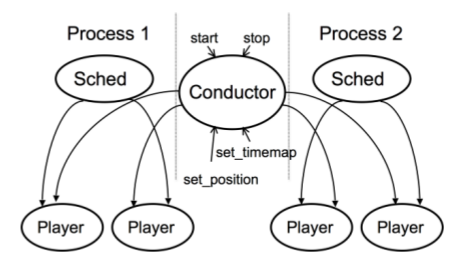
\includegraphics[width=0.65\linewidth]{1/1.png}}
\caption{Key Components of HCMP}
\label{fig:speciation}
\end{figure}
 

\section{Architecture}
\subsection{HCMP Architecture}
Figure 1.2 shows architecture of the whole HCMP project. it mainly contain 5 
subsystems. A brief description of each subsystem and its function will be
given in following paragraphs.
\begin{figure}[H] % Example image
\center{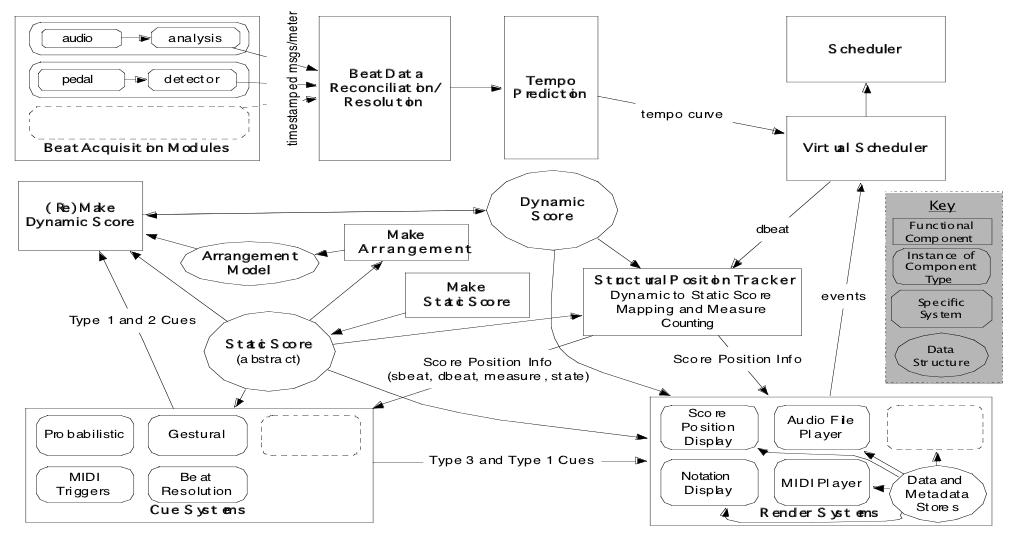
\includegraphics[width=1\linewidth]{1/2.png}}
\caption{Whole Picture of the HCMP Project}
\label{fig:speciation}
\end{figure}

\subsubsection{Real-Time System}
Real-time components are needed to keep an HCMP system coordinated with
the human musicians in an ensemble. Real-time synchronization aspects are
handled by components such as beat and tempo tracking systems.

\subsubsection{Abstract-Time System}
Abstract time components are needed to manage and schedule score events in
the context of the performance. The virtual scheduler and its associated systems are
concerned with the abstract time aspects of the system. The virtual scheduler should
reschedule events scheduled on a nominal time trajectory by warping the event times
according to the incoming tempo data from the tempo prediction system. Events are
then passed to an actual scheduler for real-time scheduling.

\subsubsection{Score and Arrangement System}
Score management is handled by the functional components in the center box of
the diagram. These systems will allow a human musician to encode, manage, and
arrange scores for performance.

\subsubsection{Cueing System}
Cueing systems are required to allow the computer system to react to high-level
structural and synchronization changes during performance (e.g. additional
repetitions of a chorus). There are mainly three types of cues:
\begin{enumerate}
  \item Static Score Position Cue. This cue is necessary when synchronization with the
static score is lost. Issuing it will cause the dynamic score to be re-made
accordingly.
  \item Intention Cue. This cue is needed to inform the computer of the intended
direction of the current performance (e.g. exiting a vamp section or adding an
additional chorus). Issuing it (e.g. using a MIDI trigger, gesture recognition or
other method) will cause the future dynamic score to be remade.
  \item Voicing/Arrangement Cue. This cue is needed to allow control over the voicing
of a section (e.g. it may be desirable to prevent a particular instrumental group
from playing on the first time through a repeat but allow them to play on the
second). Issuing this type of cue affects only the render system to which it is
issued.
\end{enumerate}

\subsubsection{Render System}
Render systems are responsible for providing different kindos multi-media output 
at the appropriate time. Render system will be designed as some kind of ``add-on'' 
for the HCMP, so that we could flexibly change, remove and update the render system.
With unified programming interface, each reander system is provided similar raw 
data and each system should also define its own way of parsing the raw data.
Sometimes, metadata is required to link these data elements to their appropriate 
static score position (and thus to
their appropriate scheduling as the dynamic score is played). A standardized
format will be required for this to relate static-score measure-numbers and the
dynamic score position and context to the properties of the format concerned. This
provide render systems more flexibility to determine how they need to deal with 
beat-level information or simply use the measure-level data, for example, a score 
display system might map a measure to image information or an audio render 
system might represent audio at the beat level.

%Abstract beat-time information can thus be linked to real-time source material
%(to allow the correct scheduling of real-time data) while allowing the overall system
%to remain oblivious to the specific source formats being used. Render systems
%should use a callback interface whereby they schedule events with the scheduling
%systems. These call the appropriate renderer at the scheduled time, causing
%synchronized real-time output of media in accordance with the dynamic score and
%beat tracking information.

\subsection{HCMP Player Architecture}
From system architectures' perspective, the interal HCMP Player is mainly made up of
two threads, we name the thread that taking
care of user input, maintaining graphic state GUI thread. And the thread worked as   
player engine is called performer thread, each thread is a independent 
module and executed in a separated thread space. Timer will be external source 
which periodically invoke the user in do some task. A timer usually come with a 
language library, so its implementation is within the category of this paper.

During the performance, the HCMP Player will act as 
the server for the conductor component, which is constantly 
receiving control messages and responding accordingly. 

\begin{figure}[H]
\center{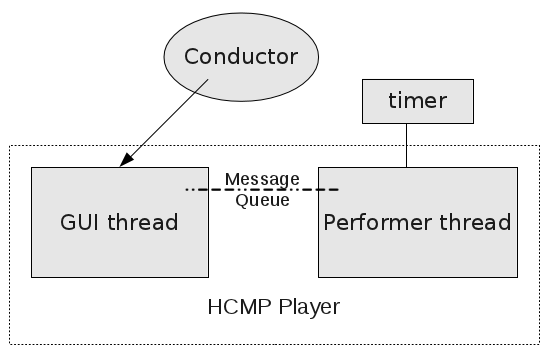
\includegraphics[width=0.65\linewidth]{2/2.png}}
\caption{Architecture of the HCMP Midi Player}
\label{fig:speciation}
\end{figure}

Internally, the Player will have two threads, with one thread for
GUI interactive control (GUI thread) and the other thread for 
performing music data (performer thread). 
The two threads will communicate with each other through a shared 
message queue, we can assume the message 
queue is large enough to avoid blocks for both caller and callee threads. 
The performaner thread
will handle time critical operations, and there will be a timer setup 
before this thread is created. The goal of the timer is to 
wake up the performer thread periodically. Everytime the performer 
thread's timer callback function is invoked, 
it will check the message queue and process any command from the control thread.
Figure 2 illustrates the overall structure of the Player.

%Most organisms use polymers of glucose units for energy storage and differ only slightly in the way they link together monomers to sometimes gigantic macromolecules. Dextran of bacteria is made from long chains of $\alpha$-1,6-linked glucose units. 

%: ----------------------- HELP: special characters
% above you can see how special characters are coded; e.g. $\alpha$
% below are the most frequently used codes:
%$\alpha$  $\beta$  $\gamma$  $\delta$

%$^{chars to be superscripted}$  OR $^x$ (for a single character)
%$_{chars to be suberscripted}$  OR $_x$

%>  $>$  greater,  <  $<$  less
%≥  $\ge$  greater than or equal, ≤  $\ge$  lesser than or equal
%~  $\sim$  similar to

%$^{\circ}$C   ° as in degree C
%±  \pm     plus/minus sign

%$\AA$     produces  Å (Angstrom)

% dextran, starch, glycogen continued
%Starch of plants and glycogen of animals consists of $\alpha$-1,4-glycosidic glucose polymers \cite{lastname07}. See figure \ref{largepotato} for a comparison of glucose polymer structure and chemistry. 

%Two references can be placed separated by a comma \cite{lastname07,name06}.

%: ----------------------- HELP: references
% References can be links to figures, tables, sections, or references.
% For figures, tables, and text you define the target of the link with \label{XYZ}. Then you call cross-link with the command \ref{XYZ}, as above
% Citations are bound in a very similar way with \cite{XYZ}. You store your references in a BibTex file with a programme like BibDesk.



%\figuremacro{largepotato}{A common glucose polymers}{The figure shows starch granules in potato cells, taken from \href{http://molecularexpressions.com/micro/gallery/burgersnfries/burgersnfries4.html}{Molecular Expressions}.}

%: ----------------------- HELP: adding figures with macros
% This template provides a very convenient way to add figures with minimal code.
% \figuremacro{1}{2}{3}{4} calls up a series of commands formating your image.
% 1 = name of the file without extension; PNG, JPEG is ok; GIF doesn't work
% 2 = title of the figure AND the name of the label for cross-linking
% 3 = caption text for the figure

%: ----------------------- HELP: www links
% You can also see above how, www links are placed
% \href{http://www.something.net}{link text}

%\figuremacroW{largepotato}{Title}{Caption}{0.8}

% variation of the above macro with a width setting
% \figuremacroW{1}{2}{3}{4}
% 1-3 as above
% 4 = size relative to text width which is 1; use this to reduce figures


%Insulin stimulates the following processes:
%
%\begin{itemize}
%\item muscle and fat cells remove glucose from the blood,
%\item cells breakdown glucose via glycolysis and the citrate cycle, storing its energy in the form of ATP,
%\item liver and muscle store glucose as glycogen as a short-term energy reserve,
%\item adipose tissue stores glucose as fat for long-term energy reserve, and
%\item cells use glucose for protein synthesis.
%\end{itemize}

%: ----------------------- HELP: lists
% This is how you generate lists in LaTeX.
% If you replace {itemize} by {enumerate} you get a numbered list.

%: ----------------------- HELP: tables
% Directly coding tables in latex is tiresome. See below.
% I would recommend using a converter macro that allows you to make the table in Excel and convert them into latex code which you can then paste into your doc.
% This is the link: http://www.softpedia.com/get/Office-tools/Other-Office-Tools/Excel2Latex.shtml
% It's a Excel template file containing a macro for the conversion.

% There you go. You already know the most important things.

\chapter{Introduction}

% the code below specifies where the figures are stored
\ifpdf
    \graphicspath{{1_introduction/figures/PNG/}{1_introduction/figures/PDF/}{1_introduction/figures/}}
\else
    \graphicspath{{1_introduction/figures/EPS/}{1_introduction/figures/}}
\fi

\section{Overview}
Computers have been widely used in music performances for many years. Some
advanced systems use the computer as a independent module to replace a
single instrument in an orchestra. In popular music computers have proved
to be particularly successful. Both classical and popular music have many
opportunities for innovative applications used by highly intelligent and
coordinated computer music systems. With more powerful algorithms and more
advanced sensing devices, computer music systems have the potential to
replace musicians. In the future, computer music systems will inspire new 
musical directions based on new
capabilities and generate new concepts from new technologies.

Live popular music offers a wealth of opportunities for computing and music
research.  We term the integration of computers as independent autonomous
performers into popular live music performances as Human Computer Music
Performance (HCMP). In HCMP computers become more than instruments and are,
in some degree, seen as performers. To bring HCMP into the realm of popular
music performance, certain problems need to be solved. 

One problem is that
popular music is organized around a tight synchronization to beats and a
computer cannot reliably and efficiently adapt to human tempo variations.
Another significant problem is that an HCMP project is a large complex
system which contain many components, each one relying on the cooperation of several
different subcomponents to complete its task.

The motivation behind the HCMP Player is to provide a good solution to these
problems. When successful, the HCMP Player will display different
representations of music, work as an accompaniment  and quickly adjust its
tempo to follow the performer. A clearly defined programming interface is
also required in order to foster communication and cooperation with all
components within the system. To create such a player, we must coordinate
time between different media. We need at least two functional components,
one component working as ``backend'' and responsible for coordinating and
scheduling different music events, the other, working as ``frontend'', will
receive commands from the user or other components and dynamically adjust
play sequence and tempo based on those requests.

This paper begins with the role of the HCMP Player in the HCMP project. Then
the ``big picture of'' of the HCMP project will be discussed, followed by a
presentation of the individual HCMP components. Finally the question that how
does the HMCP Player fit into the whole picture will be addressed. In the
following three chapters design issues with the HCMP Player are addressed.
Each chapter approaches the problem from a different perspective. Chapter 2
describes the design of Graphic User Interface (GUI) of HCMP Player together
with a detailed explanation of all the GUI components' usage and function.
Chapter 3 describes the ``backend'' of the HCMP Player - the player engine,
and illustrates how the player engine cooperates and communicates with the
GUI to complete external requests. Chapter 4 addresses the network
communication problem between multiple players. A set of unified API is
defined to make the HCMP Player compatible with other components in the HCMP
project.  Chapter 5 describes the implementation details of the HCMP Player
and includes pseucode to provide a clear explanation of this. Chapter 6
focuses on the evaluation of the HCMP Player, a full list of feature points
will be given and a clear success criteria used to evaluate the HCMP Player
will be defined.  In chapter 7, I summarize my work and propose possible
future works.

\section{Background}

Before making a formal introduction to the background of HCMP Player. 
I would like to make short review of  
some existed human computer music systems. The most common use of computer in
music performance is through computer instruments, typically keyboards.
These, and other electronic instruments, are essentially substitutes for traditional
instruments and rely upon human musicians for their control and coordination with
other musicians. Many composers of interactive contemporary art music use computers
to generate music in real time, often in response to live performers.

Another meaningful use of computer in music is computer accompaniment system 
\cite{Roger:89}, 
whcih solves the synchronization problem by assuming a pre-determined 
score (music notation). During the performance, a performer expressively 
played music score, while the accompaniment system ``listen'' and analysis, 
then follows the performer 
in the score and synchronizes an accompaniment.

In live popular music peformance, computer is quite useful too.
The computer has had a significant
impact on popular music through drum machines, sequencers and loop-based
interfaces, but one can argue that popular music has adapted to new technology
rather than the other way around. The sound and beat of drum machines seems stiff,
mechanical, and monotonous to many musicians, but that became the trance-like
foundation of club dance music and other forms . Similarly, 
the inability of
sequencers and other beat-based software to “listen” to human musicians has led to
performances with click tracks in fixed media or simply a fixed drum track that live
musicians must follow. Ableton Live \cite{Ableton:2011} is an example of software that
uses a beat, measure, and section framework to synchronize music in live
performance, but the program is not well suited to adapting to the tempo of live
musicians. Robertson and Plumbley \cite{Robertson:2007} used a real-time beat 
tracker in
conjunction with Ableton Live software to synchronize pre-recorded music 
to a live drummer. This extension could be considered HCMP.
The table 1.1 summarize some of existed computer music systems and their usage.

\begin{table}[htdp]
\centering
\begin{tabular}{| p{5cm} | p{8cm} |} % ccc means 3 columns, all centered; alternatives are l, r

\hline
Computer Instruments & Direct physical interaction with virtual instruments \\

\hline 
Interactive Contemporary Art Music & Composed interactions; often unconstrained by
traditional harmony or rhythm.\\

\hline
Computer Accompaniment & score following synchronizes computer to live performer.\\

\hline
Fixed Media  & Many musical styles and formats. Live performers
synchronize to fixed recording.\\

\hline
Conducting System & Synchronize live computer performance by tapping or
gesturing beats. Best with “expressive”
traditional/classical music.\\
\hline
\end{tabular}
\caption[Computer Music Systems Summary]{Computer Music Systems Summary}
\label{latexin_genes} % label for cross-links with \ref{latexin_genes}
\end{table}

\section{Objective}
The objective of HCMP \cite{Dawen:2011} is to create an autonomous 
``artificial performer'' with the ability of a human-level musical performance. 
Hopefully, HCMP does not require a human operator's interfere, the system itself 
is designed to be adaptive and responsive. With sophisticated listening and sensing
component, HCMP is able to adjust related system parameters in real-time during 
performance. From functional perspective, we can divide HCMP into two main
categories: music preparation and music performance. Music preparation
part aims to work and understand with multiple music representations. Music
performance part is to deal with various issues regarding to question 
how to play music.     

An important component of the music performance part is the HCMP Player, 
which is able to flexibly  
adjust and respond to changes of music signal. Figure 1 illustrates relationship 
between scheduler, conductor and HCMP Plyaer. During performance, the HCMP Player will 
be controlled by conductor and constantly receive control messages 
from its conductor. In this project, I will design, implement the HCMP midi player 
for the HCMP project that is able to fully cooperate with conductor and scheduler.
\begin{figure}[H] % Example image
\center{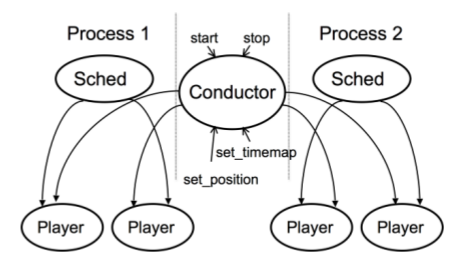
\includegraphics[width=0.65\linewidth]{1/1.png}}
\caption{Key Components of HCMP}
\label{fig:speciation}
\end{figure}
 

\section{Architecture}
\subsection{HCMP Architecture}
Figure 1.2 shows architecture of the whole HCMP project. it mainly contain 5 
subsystems. A brief description of each subsystem and its function will be
given in following paragraphs.
\begin{figure}[H] % Example image
\center{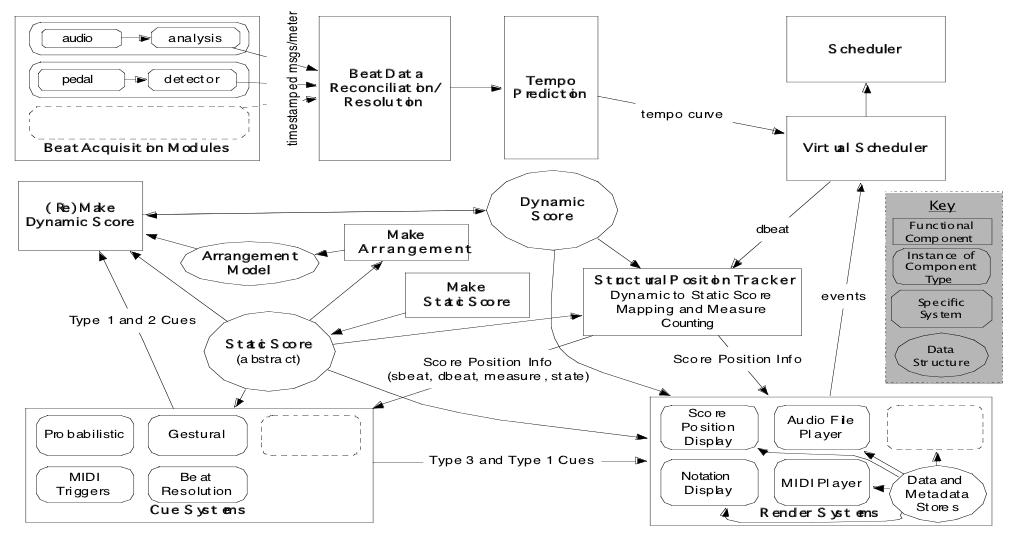
\includegraphics[width=1\linewidth]{1/2.png}}
\caption{Whole Picture of the HCMP Project}
\label{fig:speciation}
\end{figure}

\subsubsection{Real-Time System}
Real-time components are needed to keep an HCMP system coordinated with
the human musicians in an ensemble. Real-time synchronization aspects are
handled by components such as beat and tempo tracking systems.

\subsubsection{Abstract-Time System}
Abstract time components are needed to manage and schedule score events in
the context of the performance. The virtual scheduler and its associated systems are
concerned with the abstract time aspects of the system. The virtual scheduler should
reschedule events scheduled on a nominal time trajectory by warping the event times
according to the incoming tempo data from the tempo prediction system. Events are
then passed to an actual scheduler for real-time scheduling.

\subsubsection{Score and Arrangement System}
Score management is handled by the functional components in the center box of
the diagram. These systems will allow a human musician to encode, manage, and
arrange scores for performance.

\subsubsection{Cueing System}
Cueing systems are required to allow the computer system to react to high-level
structural and synchronization changes during performance (e.g. additional
repetitions of a chorus). There are mainly three types of cues:
\begin{enumerate}
  \item Static Score Position Cue. This cue is necessary when synchronization with the
static score is lost. Issuing it will cause the dynamic score to be re-made
accordingly.
  \item Intention Cue. This cue is needed to inform the computer of the intended
direction of the current performance (e.g. exiting a vamp section or adding an
additional chorus). Issuing it (e.g. using a MIDI trigger, gesture recognition or
other method) will cause the future dynamic score to be remade.
  \item Voicing/Arrangement Cue. This cue is needed to allow control over the voicing
of a section (e.g. it may be desirable to prevent a particular instrumental group
from playing on the first time through a repeat but allow them to play on the
second). Issuing this type of cue affects only the render system to which it is
issued.
\end{enumerate}

\subsubsection{Render System}
Render systems are responsible for providing different kindos multi-media output 
at the appropriate time. Render system will be designed as some kind of ``add-on'' 
for the HCMP, so that we could flexibly change, remove and update the render system.
With unified programming interface, each reander system is provided similar raw 
data and each system should also define its own way of parsing the raw data.
Sometimes, metadata is required to link these data elements to their appropriate 
static score position (and thus to
their appropriate scheduling as the dynamic score is played). A standardized
format will be required for this to relate static-score measure-numbers and the
dynamic score position and context to the properties of the format concerned. This
provide render systems more flexibility to determine how they need to deal with 
beat-level information or simply use the measure-level data, for example, a score 
display system might map a measure to image information or an audio render 
system might represent audio at the beat level.

%Abstract beat-time information can thus be linked to real-time source material
%(to allow the correct scheduling of real-time data) while allowing the overall system
%to remain oblivious to the specific source formats being used. Render systems
%should use a callback interface whereby they schedule events with the scheduling
%systems. These call the appropriate renderer at the scheduled time, causing
%synchronized real-time output of media in accordance with the dynamic score and
%beat tracking information.

\subsection{HCMP Player Architecture}
From system architectures' perspective, the interal HCMP Player is mainly made up of
two threads, we name the thread that taking
care of user input, maintaining graphic state GUI thread. And the thread worked as   
player engine is called performer thread, each thread is a independent 
module and executed in a separated thread space. Timer will be external source 
which periodically invoke the user in do some task. A timer usually come with a 
language library, so its implementation is within the category of this paper.

During the performance, the HCMP Player will act as 
the server for the conductor component, which is constantly 
receiving control messages and responding accordingly. 

\begin{figure}[H]
\center{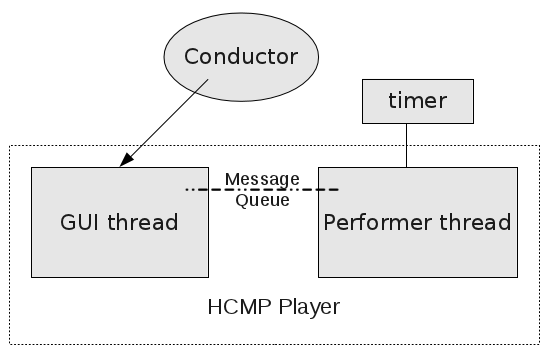
\includegraphics[width=0.65\linewidth]{2/2.png}}
\caption{Architecture of the HCMP Midi Player}
\label{fig:speciation}
\end{figure}

Internally, the Player will have two threads, with one thread for
GUI interactive control (GUI thread) and the other thread for 
performing music data (performer thread). 
The two threads will communicate with each other through a shared 
message queue, we can assume the message 
queue is large enough to avoid blocks for both caller and callee threads. 
The performaner thread
will handle time critical operations, and there will be a timer setup 
before this thread is created. The goal of the timer is to 
wake up the performer thread periodically. Everytime the performer 
thread's timer callback function is invoked, 
it will check the message queue and process any command from the control thread.
Figure 2 illustrates the overall structure of the Player.

%Most organisms use polymers of glucose units for energy storage and differ only slightly in the way they link together monomers to sometimes gigantic macromolecules. Dextran of bacteria is made from long chains of $\alpha$-1,6-linked glucose units. 

%: ----------------------- HELP: special characters
% above you can see how special characters are coded; e.g. $\alpha$
% below are the most frequently used codes:
%$\alpha$  $\beta$  $\gamma$  $\delta$

%$^{chars to be superscripted}$  OR $^x$ (for a single character)
%$_{chars to be suberscripted}$  OR $_x$

%>  $>$  greater,  <  $<$  less
%≥  $\ge$  greater than or equal, ≤  $\ge$  lesser than or equal
%~  $\sim$  similar to

%$^{\circ}$C   ° as in degree C
%±  \pm     plus/minus sign

%$\AA$     produces  Å (Angstrom)

% dextran, starch, glycogen continued
%Starch of plants and glycogen of animals consists of $\alpha$-1,4-glycosidic glucose polymers \cite{lastname07}. See figure \ref{largepotato} for a comparison of glucose polymer structure and chemistry. 

%Two references can be placed separated by a comma \cite{lastname07,name06}.

%: ----------------------- HELP: references
% References can be links to figures, tables, sections, or references.
% For figures, tables, and text you define the target of the link with \label{XYZ}. Then you call cross-link with the command \ref{XYZ}, as above
% Citations are bound in a very similar way with \cite{XYZ}. You store your references in a BibTex file with a programme like BibDesk.



%\figuremacro{largepotato}{A common glucose polymers}{The figure shows starch granules in potato cells, taken from \href{http://molecularexpressions.com/micro/gallery/burgersnfries/burgersnfries4.html}{Molecular Expressions}.}

%: ----------------------- HELP: adding figures with macros
% This template provides a very convenient way to add figures with minimal code.
% \figuremacro{1}{2}{3}{4} calls up a series of commands formating your image.
% 1 = name of the file without extension; PNG, JPEG is ok; GIF doesn't work
% 2 = title of the figure AND the name of the label for cross-linking
% 3 = caption text for the figure

%: ----------------------- HELP: www links
% You can also see above how, www links are placed
% \href{http://www.something.net}{link text}

%\figuremacroW{largepotato}{Title}{Caption}{0.8}

% variation of the above macro with a width setting
% \figuremacroW{1}{2}{3}{4}
% 1-3 as above
% 4 = size relative to text width which is 1; use this to reduce figures


%Insulin stimulates the following processes:
%
%\begin{itemize}
%\item muscle and fat cells remove glucose from the blood,
%\item cells breakdown glucose via glycolysis and the citrate cycle, storing its energy in the form of ATP,
%\item liver and muscle store glucose as glycogen as a short-term energy reserve,
%\item adipose tissue stores glucose as fat for long-term energy reserve, and
%\item cells use glucose for protein synthesis.
%\end{itemize}

%: ----------------------- HELP: lists
% This is how you generate lists in LaTeX.
% If you replace {itemize} by {enumerate} you get a numbered list.

%: ----------------------- HELP: tables
% Directly coding tables in latex is tiresome. See below.
% I would recommend using a converter macro that allows you to make the table in Excel and convert them into latex code which you can then paste into your doc.
% This is the link: http://www.softpedia.com/get/Office-tools/Other-Office-Tools/Excel2Latex.shtml
% It's a Excel template file containing a macro for the conversion.

% There you go. You already know the most important things.

\chapter{Introduction}

% the code below specifies where the figures are stored
\ifpdf
    \graphicspath{{1_introduction/figures/PNG/}{1_introduction/figures/PDF/}{1_introduction/figures/}}
\else
    \graphicspath{{1_introduction/figures/EPS/}{1_introduction/figures/}}
\fi

\section{Overview}
Computers have been widely used in music performances for many years. Some
advanced systems use the computer as a independent module to replace a
single instrument in an orchestra. In popular music computers have proved
to be particularly successful. Both classical and popular music have many
opportunities for innovative applications used by highly intelligent and
coordinated computer music systems. With more powerful algorithms and more
advanced sensing devices, computer music systems have the potential to
replace musicians. In the future, computer music systems will inspire new 
musical directions based on new
capabilities and generate new concepts from new technologies.

Live popular music offers a wealth of opportunities for computing and music
research.  We term the integration of computers as independent autonomous
performers into popular live music performances as Human Computer Music
Performance (HCMP). In HCMP computers become more than instruments and are,
in some degree, seen as performers. To bring HCMP into the realm of popular
music performance, certain problems need to be solved. 

One problem is that
popular music is organized around a tight synchronization to beats and a
computer cannot reliably and efficiently adapt to human tempo variations.
Another significant problem is that an HCMP project is a large complex
system which contain many components, each one relying on the cooperation of several
different subcomponents to complete its task.

The motivation behind the HCMP Player is to provide a good solution to these
problems. When successful, the HCMP Player will display different
representations of music, work as an accompaniment  and quickly adjust its
tempo to follow the performer. A clearly defined programming interface is
also required in order to foster communication and cooperation with all
components within the system. To create such a player, we must coordinate
time between different media. We need at least two functional components,
one component working as ``backend'' and responsible for coordinating and
scheduling different music events, the other, working as ``frontend'', will
receive commands from the user or other components and dynamically adjust
play sequence and tempo based on those requests.

This paper begins with the role of the HCMP Player in the HCMP project. Then
the ``big picture of'' of the HCMP project will be discussed, followed by a
presentation of the individual HCMP components. Finally the question that how
does the HMCP Player fit into the whole picture will be addressed. In the
following three chapters design issues with the HCMP Player are addressed.
Each chapter approaches the problem from a different perspective. Chapter 2
describes the design of Graphic User Interface (GUI) of HCMP Player together
with a detailed explanation of all the GUI components' usage and function.
Chapter 3 describes the ``backend'' of the HCMP Player - the player engine,
and illustrates how the player engine cooperates and communicates with the
GUI to complete external requests. Chapter 4 addresses the network
communication problem between multiple players. A set of unified API is
defined to make the HCMP Player compatible with other components in the HCMP
project.  Chapter 5 describes the implementation details of the HCMP Player
and includes pseucode to provide a clear explanation of this. Chapter 6
focuses on the evaluation of the HCMP Player, a full list of feature points
will be given and a clear success criteria used to evaluate the HCMP Player
will be defined.  In chapter 7, I summarize my work and propose possible
future works.

\section{Background}

Before making a formal introduction to the background of HCMP Player. 
I would like to make short review of  
some existed human computer music systems. The most common use of computer in
music performance is through computer instruments, typically keyboards.
These, and other electronic instruments, are essentially substitutes for traditional
instruments and rely upon human musicians for their control and coordination with
other musicians. Many composers of interactive contemporary art music use computers
to generate music in real time, often in response to live performers.

Another meaningful use of computer in music is computer accompaniment system 
\cite{Roger:89}, 
whcih solves the synchronization problem by assuming a pre-determined 
score (music notation). During the performance, a performer expressively 
played music score, while the accompaniment system ``listen'' and analysis, 
then follows the performer 
in the score and synchronizes an accompaniment.

In live popular music peformance, computer is quite useful too.
The computer has had a significant
impact on popular music through drum machines, sequencers and loop-based
interfaces, but one can argue that popular music has adapted to new technology
rather than the other way around. The sound and beat of drum machines seems stiff,
mechanical, and monotonous to many musicians, but that became the trance-like
foundation of club dance music and other forms . Similarly, 
the inability of
sequencers and other beat-based software to “listen” to human musicians has led to
performances with click tracks in fixed media or simply a fixed drum track that live
musicians must follow. Ableton Live \cite{Ableton:2011} is an example of software that
uses a beat, measure, and section framework to synchronize music in live
performance, but the program is not well suited to adapting to the tempo of live
musicians. Robertson and Plumbley \cite{Robertson:2007} used a real-time beat 
tracker in
conjunction with Ableton Live software to synchronize pre-recorded music 
to a live drummer. This extension could be considered HCMP.
The table 1.1 summarize some of existed computer music systems and their usage.

\begin{table}[htdp]
\centering
\begin{tabular}{| p{5cm} | p{8cm} |} % ccc means 3 columns, all centered; alternatives are l, r

\hline
Computer Instruments & Direct physical interaction with virtual instruments \\

\hline 
Interactive Contemporary Art Music & Composed interactions; often unconstrained by
traditional harmony or rhythm.\\

\hline
Computer Accompaniment & score following synchronizes computer to live performer.\\

\hline
Fixed Media  & Many musical styles and formats. Live performers
synchronize to fixed recording.\\

\hline
Conducting System & Synchronize live computer performance by tapping or
gesturing beats. Best with “expressive”
traditional/classical music.\\
\hline
\end{tabular}
\caption[Computer Music Systems Summary]{Computer Music Systems Summary}
\label{latexin_genes} % label for cross-links with \ref{latexin_genes}
\end{table}

\section{Objective}
The objective of HCMP \cite{Dawen:2011} is to create an autonomous 
``artificial performer'' with the ability of a human-level musical performance. 
Hopefully, HCMP does not require a human operator's interfere, the system itself 
is designed to be adaptive and responsive. With sophisticated listening and sensing
component, HCMP is able to adjust related system parameters in real-time during 
performance. From functional perspective, we can divide HCMP into two main
categories: music preparation and music performance. Music preparation
part aims to work and understand with multiple music representations. Music
performance part is to deal with various issues regarding to question 
how to play music.     

An important component of the music performance part is the HCMP Player, 
which is able to flexibly  
adjust and respond to changes of music signal. Figure 1 illustrates relationship 
between scheduler, conductor and HCMP Plyaer. During performance, the HCMP Player will 
be controlled by conductor and constantly receive control messages 
from its conductor. In this project, I will design, implement the HCMP midi player 
for the HCMP project that is able to fully cooperate with conductor and scheduler.
\begin{figure}[H] % Example image
\center{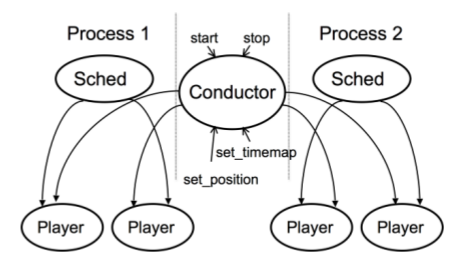
\includegraphics[width=0.65\linewidth]{1/1.png}}
\caption{Key Components of HCMP}
\label{fig:speciation}
\end{figure}
 

\section{Architecture}
\subsection{HCMP Architecture}
Figure 1.2 shows architecture of the whole HCMP project. it mainly contain 5 
subsystems. A brief description of each subsystem and its function will be
given in following paragraphs.
\begin{figure}[H] % Example image
\center{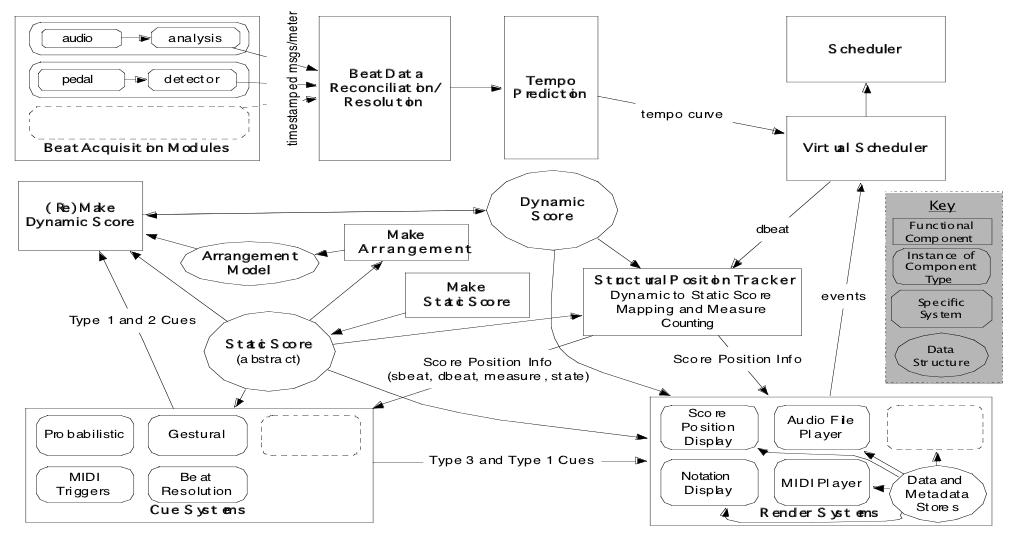
\includegraphics[width=1\linewidth]{1/2.png}}
\caption{Whole Picture of the HCMP Project}
\label{fig:speciation}
\end{figure}

\subsubsection{Real-Time System}
Real-time components are needed to keep an HCMP system coordinated with
the human musicians in an ensemble. Real-time synchronization aspects are
handled by components such as beat and tempo tracking systems.

\subsubsection{Abstract-Time System}
Abstract time components are needed to manage and schedule score events in
the context of the performance. The virtual scheduler and its associated systems are
concerned with the abstract time aspects of the system. The virtual scheduler should
reschedule events scheduled on a nominal time trajectory by warping the event times
according to the incoming tempo data from the tempo prediction system. Events are
then passed to an actual scheduler for real-time scheduling.

\subsubsection{Score and Arrangement System}
Score management is handled by the functional components in the center box of
the diagram. These systems will allow a human musician to encode, manage, and
arrange scores for performance.

\subsubsection{Cueing System}
Cueing systems are required to allow the computer system to react to high-level
structural and synchronization changes during performance (e.g. additional
repetitions of a chorus). There are mainly three types of cues:
\begin{enumerate}
  \item Static Score Position Cue. This cue is necessary when synchronization with the
static score is lost. Issuing it will cause the dynamic score to be re-made
accordingly.
  \item Intention Cue. This cue is needed to inform the computer of the intended
direction of the current performance (e.g. exiting a vamp section or adding an
additional chorus). Issuing it (e.g. using a MIDI trigger, gesture recognition or
other method) will cause the future dynamic score to be remade.
  \item Voicing/Arrangement Cue. This cue is needed to allow control over the voicing
of a section (e.g. it may be desirable to prevent a particular instrumental group
from playing on the first time through a repeat but allow them to play on the
second). Issuing this type of cue affects only the render system to which it is
issued.
\end{enumerate}

\subsubsection{Render System}
Render systems are responsible for providing different kindos multi-media output 
at the appropriate time. Render system will be designed as some kind of ``add-on'' 
for the HCMP, so that we could flexibly change, remove and update the render system.
With unified programming interface, each reander system is provided similar raw 
data and each system should also define its own way of parsing the raw data.
Sometimes, metadata is required to link these data elements to their appropriate 
static score position (and thus to
their appropriate scheduling as the dynamic score is played). A standardized
format will be required for this to relate static-score measure-numbers and the
dynamic score position and context to the properties of the format concerned. This
provide render systems more flexibility to determine how they need to deal with 
beat-level information or simply use the measure-level data, for example, a score 
display system might map a measure to image information or an audio render 
system might represent audio at the beat level.

%Abstract beat-time information can thus be linked to real-time source material
%(to allow the correct scheduling of real-time data) while allowing the overall system
%to remain oblivious to the specific source formats being used. Render systems
%should use a callback interface whereby they schedule events with the scheduling
%systems. These call the appropriate renderer at the scheduled time, causing
%synchronized real-time output of media in accordance with the dynamic score and
%beat tracking information.

\subsection{HCMP Player Architecture}
From system architectures' perspective, the interal HCMP Player is mainly made up of
two threads, we name the thread that taking
care of user input, maintaining graphic state GUI thread. And the thread worked as   
player engine is called performer thread, each thread is a independent 
module and executed in a separated thread space. Timer will be external source 
which periodically invoke the user in do some task. A timer usually come with a 
language library, so its implementation is within the category of this paper.

During the performance, the HCMP Player will act as 
the server for the conductor component, which is constantly 
receiving control messages and responding accordingly. 

\begin{figure}[H]
\center{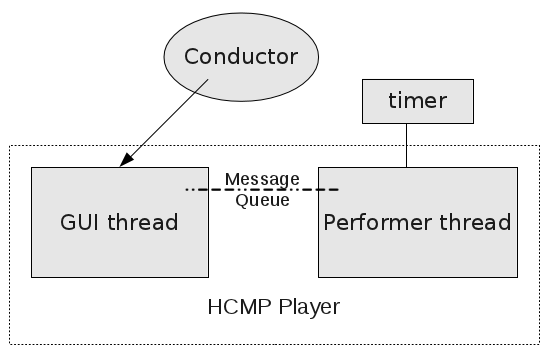
\includegraphics[width=0.65\linewidth]{2/2.png}}
\caption{Architecture of the HCMP Midi Player}
\label{fig:speciation}
\end{figure}

Internally, the Player will have two threads, with one thread for
GUI interactive control (GUI thread) and the other thread for 
performing music data (performer thread). 
The two threads will communicate with each other through a shared 
message queue, we can assume the message 
queue is large enough to avoid blocks for both caller and callee threads. 
The performaner thread
will handle time critical operations, and there will be a timer setup 
before this thread is created. The goal of the timer is to 
wake up the performer thread periodically. Everytime the performer 
thread's timer callback function is invoked, 
it will check the message queue and process any command from the control thread.
Figure 2 illustrates the overall structure of the Player.

%Most organisms use polymers of glucose units for energy storage and differ only slightly in the way they link together monomers to sometimes gigantic macromolecules. Dextran of bacteria is made from long chains of $\alpha$-1,6-linked glucose units. 

%: ----------------------- HELP: special characters
% above you can see how special characters are coded; e.g. $\alpha$
% below are the most frequently used codes:
%$\alpha$  $\beta$  $\gamma$  $\delta$

%$^{chars to be superscripted}$  OR $^x$ (for a single character)
%$_{chars to be suberscripted}$  OR $_x$

%>  $>$  greater,  <  $<$  less
%≥  $\ge$  greater than or equal, ≤  $\ge$  lesser than or equal
%~  $\sim$  similar to

%$^{\circ}$C   ° as in degree C
%±  \pm     plus/minus sign

%$\AA$     produces  Å (Angstrom)

% dextran, starch, glycogen continued
%Starch of plants and glycogen of animals consists of $\alpha$-1,4-glycosidic glucose polymers \cite{lastname07}. See figure \ref{largepotato} for a comparison of glucose polymer structure and chemistry. 

%Two references can be placed separated by a comma \cite{lastname07,name06}.

%: ----------------------- HELP: references
% References can be links to figures, tables, sections, or references.
% For figures, tables, and text you define the target of the link with \label{XYZ}. Then you call cross-link with the command \ref{XYZ}, as above
% Citations are bound in a very similar way with \cite{XYZ}. You store your references in a BibTex file with a programme like BibDesk.



%\figuremacro{largepotato}{A common glucose polymers}{The figure shows starch granules in potato cells, taken from \href{http://molecularexpressions.com/micro/gallery/burgersnfries/burgersnfries4.html}{Molecular Expressions}.}

%: ----------------------- HELP: adding figures with macros
% This template provides a very convenient way to add figures with minimal code.
% \figuremacro{1}{2}{3}{4} calls up a series of commands formating your image.
% 1 = name of the file without extension; PNG, JPEG is ok; GIF doesn't work
% 2 = title of the figure AND the name of the label for cross-linking
% 3 = caption text for the figure

%: ----------------------- HELP: www links
% You can also see above how, www links are placed
% \href{http://www.something.net}{link text}

%\figuremacroW{largepotato}{Title}{Caption}{0.8}

% variation of the above macro with a width setting
% \figuremacroW{1}{2}{3}{4}
% 1-3 as above
% 4 = size relative to text width which is 1; use this to reduce figures


%Insulin stimulates the following processes:
%
%\begin{itemize}
%\item muscle and fat cells remove glucose from the blood,
%\item cells breakdown glucose via glycolysis and the citrate cycle, storing its energy in the form of ATP,
%\item liver and muscle store glucose as glycogen as a short-term energy reserve,
%\item adipose tissue stores glucose as fat for long-term energy reserve, and
%\item cells use glucose for protein synthesis.
%\end{itemize}

%: ----------------------- HELP: lists
% This is how you generate lists in LaTeX.
% If you replace {itemize} by {enumerate} you get a numbered list.

%: ----------------------- HELP: tables
% Directly coding tables in latex is tiresome. See below.
% I would recommend using a converter macro that allows you to make the table in Excel and convert them into latex code which you can then paste into your doc.
% This is the link: http://www.softpedia.com/get/Office-tools/Other-Office-Tools/Excel2Latex.shtml
% It's a Excel template file containing a macro for the conversion.

% There you go. You already know the most important things.


\bibliographystyle{Latex/Classes/PhDbiblio-url2}
\renewcommand{\bibname}{References}
\bibliography{9/references}


% Thesis statement of originality -------------------------------------

\begin{declaration}        %this creates the heading for the declaration page

I herewith declare that I have produced this paper without the prohibited 
assistance of third parties and without making use of aids other than those specified; 
This paper has not previously been presented in identical or similar form to any 
other foreign examination board.

The thesis work was conducted from 02/14/2013 to 05/15/2013 under the supervision 
of Prof. Roger B. Dannenberg at Carnegie Mellon University.

\vspace{10mm}
Signature: 

\end{declaration}


% ----------------------------------------------------------------------


\end{document}

